%%%%%%%%%%%%%%%%%%%%%%%%%%%%%%%%%%%%%%%%%%%%%%%%%%%%%%%%%%%%%%%%%%%%%%%%%%%%%%%%
%% Comprehensive QuantLib Derivatives Pricing Lecture
%% A 200-Slide Technical Deep Dive
%% From Basic Swaps to Callable Cross-Currency Exotic Derivatives
%%%%%%%%%%%%%%%%%%%%%%%%%%%%%%%%%%%%%%%%%%%%%%%%%%%%%%%%%%%%%%%%%%%%%%%%%%%%%%%%

\documentclass[aspectratio=169,11pt]{beamer}

\usepackage[T1]{fontenc}
\usepackage[utf8]{inputenc}
\usepackage{lmodern}
\usepackage{mastering_ir_derivatives_beamer_1.0}
\usepackage{booktabs}
\usepackage{array}
\usepackage{listings}

% Retain the supplied visual system without changing the authored slide count.
\beamerdefaultoverlayspecification{<*>}
\AtBeginSection[]{}
\AtBeginSubsection[]{}

\hypersetup{
    colorlinks=true,
    linkcolor=blue,
    urlcolor=blue
}

\lstset{
    basicstyle=\ttfamily\scriptsize,
    breaklines=true,
    columns=fullflexible
}

\newcommand{\product}{TGIR QuantLib Tools}
\newcommand{\code}[1]{\texttt{#1}}
\newcommand{\docdate}{2026-04-06}


% Packages
\usepackage[utf8]{inputenc}
\usepackage{amsmath,amssymb,amsthm}
\usepackage{graphicx}
\usepackage{booktabs}
\usepackage{listings}
\usepackage{tikz}
\usepackage{xcolor}
\usepackage{multicol}

% Code listing style
\lstset{
    language=Python,
    basicstyle=\ttfamily\scriptsize,
    keywordstyle=\color{blue}\bfseries,
    commentstyle=\color{green!50!black},
    stringstyle=\color{red},
    showstringspaces=false,
    breaklines=true,
    frame=single,
    backgroundcolor=\color{gray!10}
}

% Custom colors
\definecolor{quantlib}{RGB}{0,102,153}
\definecolor{python}{RGB}{53,114,165}

% Title information
\title[QuantLib Derivatives Pricing]{\textbf{Quantitative Finance with QuantLib}}
\subtitle{From Basic Swaps to Callable Cross-Currency Derivatives\\A Comprehensive Technical Journey}
\author{Quantitative Analytics Team}
\institute{TGIR QuantLib Tools Project}
\date{August 2026}

\begin{document}

%%%%%%%%%%%%%%%%%%%%%%%%%%%%%%%%%%%%%%%%%%%%%%%%%%%%%%%%%%%%%%%%%%%%%%%%%%%%%%%%
%% PART 1: INTRODUCTION AND FOUNDATIONS (Slides 1-25)
%%%%%%%%%%%%%%%%%%%%%%%%%%%%%%%%%%%%%%%%%%%%%%%%%%%%%%%%%%%%%%%%%%%%%%%%%%%%%%%%

\begin{frame}
\titlepage
\end{frame}

\begin{frame}{Lecture Overview}
\begin{columns}
\column{0.5\textwidth}
\textbf{Part I: Foundations}
\begin{itemize}
    \item Financial Derivatives Basics
    \item Time Value of Money
    \item Yield Curves
    \item QuantLib Introduction
\end{itemize}

\textbf{Part II: Interest Rate Products}
\begin{itemize}
    \item Interest Rate Swaps
    \item SOFR and OIS Markets
    \item European Swaptions
    \item Bermudan Swaptions
\end{itemize}

\column{0.5\textwidth}
\textbf{Part III: Cross-Currency \& Exotics}
\begin{itemize}
    \item FX Derivatives Basics
    \item Cross-Currency Swaps
    \item Callable XCCY Structures
    \item Three-Factor Models
\end{itemize}

\textbf{Part IV: Implementation}
\begin{itemize}
    \item Monte Carlo Methods
    \item LSM Algorithm
    \item QuantLib Architecture
    \item C++ vs Python
\end{itemize}
\end{columns}
\end{frame}

\begin{frame}{Project Timeline: A Chronological Journey}
\begin{center}
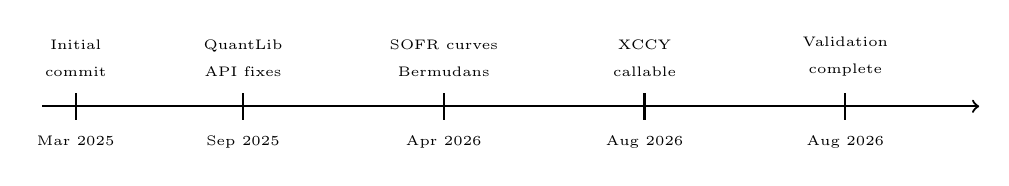
\begin{tikzpicture}[scale=0.85]
    % Timeline
    \draw[thick,->] (0,0) -- (14,0);

    % Markers
    \draw[thick] (0.5,-0.2) -- (0.5,0.2);
    \node[below] at (0.5,-0.3) {\tiny Mar 2025};
    \node[above,align=center] at (0.5,0.3) {\tiny Initial\\[-0.5ex]\tiny commit};

    \draw[thick] (3,-0.2) -- (3,0.2);
    \node[below] at (3,-0.3) {\tiny Sep 2025};
    \node[above,align=center] at (3,0.3) {\tiny QuantLib\\[-0.5ex]\tiny API fixes};

    \draw[thick] (6,-0.2) -- (6,0.2);
    \node[below] at (6,-0.3) {\tiny Apr 2026};
    \node[above,align=center] at (6,0.3) {\tiny SOFR curves\\[-0.5ex]\tiny Bermudans};

    \draw[thick] (9,-0.2) -- (9,0.2);
    \node[below] at (9,-0.3) {\tiny Aug 2026};
    \node[above,align=center] at (9,0.3) {\tiny XCCY\\[-0.5ex]\tiny callable};

    \draw[thick] (12,-0.2) -- (12,0.2);
    \node[below] at (12,-0.3) {\tiny Aug 2026};
    \node[above,align=center] at (12,0.3) {\tiny Validation\\[-0.5ex]\tiny complete};
\end{tikzpicture}
\end{center}

\vspace{0.5cm}
\textbf{Key Milestones:}
\begin{itemize}
    \item \textbf{March 2025:} Initial GPT-4.5 prototype with basic swap pricing
    \item \textbf{September 2025:} QuantLib API compatibility updates
    \item \textbf{April 2026:} SOFR curve bootstrap, Bermudan swaption engine
    \item \textbf{August 2026:} Three-factor callable XCCY with LSM Monte Carlo
\end{itemize}
\end{frame}

\begin{frame}{What is a Financial Derivative?}
\begin{block}{Definition}
A \textbf{derivative} is a financial contract whose value is \emph{derived} from an underlying asset, rate, or index.
\end{block}

\vspace{0.3cm}
\textbf{Common Underlying Assets:}
\begin{itemize}
    \item \textbf{Interest Rates:} SOFR, ESTR, Treasury yields
    \item \textbf{Equities:} Stock prices, indices (S\&P 500)
    \item \textbf{Foreign Exchange:} Currency pairs (EUR/USD)
    \item \textbf{Commodities:} Oil, gold, agricultural products
    \item \textbf{Credit:} Default probabilities, credit spreads
\end{itemize}

\vspace{0.3cm}
\textbf{Purpose:}
\begin{itemize}
    \item Hedging existing exposures
    \item Speculation on price movements
    \item Arbitrage opportunities
    \item Access to markets/payoffs otherwise unavailable
\end{itemize}
\end{frame}

\begin{frame}{Types of Derivatives}
\begin{columns}
\column{0.5\textwidth}
\textbf{Linear Derivatives}
\begin{itemize}
    \item Forwards
    \item Futures
    \item Swaps
\end{itemize}
Payoff is linear in the underlying.

\vspace{0.5cm}
\textbf{Non-Linear Derivatives}
\begin{itemize}
    \item Options (calls, puts)
    \item Caps/Floors
    \item Swaptions
\end{itemize}
Payoff has optionality (asymmetric).

\column{0.5\textwidth}
\textbf{Vanilla vs Exotic}
\begin{itemize}
    \item \textbf{Vanilla:} Standard, liquid, exchange-traded
    \item \textbf{Exotic:} Complex payoffs, OTC, bespoke
\end{itemize}

\vspace{0.5cm}
\textbf{Exotic Examples:}
\begin{itemize}
    \item Barrier options
    \item Asian options (averaging)
    \item Bermudan exercise
    \item Callable/puttable structures
    \item Cross-currency hybrids
\end{itemize}
\end{columns}
\end{frame}

\begin{frame}{Time Value of Money: Foundation of Pricing}
\begin{block}{Present Value}
\$1 today is worth more than \$1 in the future due to:
\begin{itemize}
    \item Opportunity cost (investment returns)
    \item Inflation
    \item Risk/uncertainty
\end{itemize}
\end{block}

\textbf{Discount Factor:}
\[
D(0,T) = \frac{1}{(1+r)^T} \quad \text{(discrete)}
\]
\[
D(0,T) = e^{-rT} \quad \text{(continuous)}
\]

\textbf{Present Value of Future Cashflow:}
\[
PV = \sum_{i=1}^{n} CF_i \times D(0, t_i)
\]

\vspace{0.3cm}
\emph{All derivative pricing reduces to computing expected discounted cashflows.}
\end{frame}

\begin{frame}{Yield Curves: The Term Structure of Interest Rates}
\begin{columns}
\column{0.55\textwidth}
\textbf{What is a Yield Curve?}

A yield curve shows how interest rates vary with maturity (term).

\vspace{0.3cm}
\textbf{Typical Shapes:}
\begin{itemize}
    \item \textbf{Normal:} Upward sloping (short $<$ long)
    \item \textbf{Inverted:} Downward sloping (short $>$ long)
    \item \textbf{Flat:} Similar rates across maturities
    \item \textbf{Humped:} Peak in middle maturities
\end{itemize}

\column{0.45\textwidth}
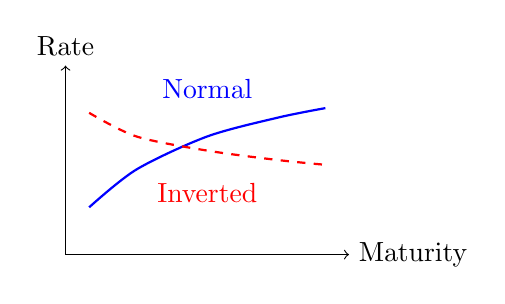
\begin{tikzpicture}[scale=0.6]
    \draw[->] (0,0) -- (6,0) node[right] {Maturity};
    \draw[->] (0,0) -- (0,4) node[above] {Rate};
    \draw[thick,blue] plot[smooth] coordinates {(0.5,1) (1.5,1.8) (3,2.5) (4.5,2.9) (5.5,3.1)};
    \node[blue] at (3,3.5) {Normal};
    \draw[thick,red,dashed] plot[smooth] coordinates {(0.5,3) (1.5,2.5) (3,2.2) (4.5,2) (5.5,1.9)};
    \node[red] at (3,1.3) {Inverted};
\end{tikzpicture}
\end{columns}

\vspace{0.3cm}
\textbf{Key Concept:} Derivatives are priced using \emph{risk-free} discount curves, typically derived from government bonds or overnight index swaps (OIS).
\end{frame}

\begin{frame}{From LIBOR to SOFR: The Rate Reform}
\begin{block}{The LIBOR Scandal and Reform}
LIBOR (London Interbank Offered Rate) was phased out due to manipulation scandals and lack of underlying transactions.
\end{block}

\textbf{New Risk-Free Rates (RFRs):}
\begin{itemize}
    \item \textbf{SOFR} (Secured Overnight Financing Rate) - USD
    \item \textbf{ESTR/€STR} (Euro Short-Term Rate) - EUR
    \item \textbf{SONIA} (Sterling Overnight Index Average) - GBP
    \item \textbf{TONA} (Tokyo Overnight Average Rate) - JPY
\end{itemize}

\textbf{Key Differences from LIBOR:}
\begin{itemize}
    \item Overnight rates (not term rates)
    \item Transaction-based (not survey-based)
    \item Near risk-free (secured or central bank)
    \item Compounded in arrears for term periods
\end{itemize}
\end{frame}

\begin{frame}{Overnight Index Swaps (OIS)}
\begin{block}{Definition}
An OIS is a swap where one party pays a fixed rate and receives the compounded overnight rate over the swap period.
\end{block}

\textbf{Structure:}
\begin{itemize}
    \item Fixed Leg: Pay fixed rate $K$ on notional $N$
    \item Floating Leg: Receive daily compounded SOFR
\end{itemize}

\textbf{SOFR Compounding:}
\[
\text{Floating Payment} = N \times \left[ \prod_{i=1}^{n} \left(1 + r_i \times \frac{d_i}{360}\right) - 1 \right]
\]

Where $r_i$ is the daily SOFR rate and $d_i$ is the day count.

\vspace{0.3cm}
\textbf{Importance:} OIS rates are used to construct the \emph{discount curve} for derivative pricing.
\end{frame}

\begin{frame}{Introduction to QuantLib}
\begin{columns}
\column{0.6\textwidth}
\textbf{What is QuantLib?}
\begin{itemize}
    \item Open-source C++ library for quantitative finance
    \item Started in 2000, mature and widely used
    \item Covers interest rates, equity, FX, credit
    \item Python bindings via SWIG (QuantLib-Python)
\end{itemize}

\vspace{0.3cm}
\textbf{Why QuantLib?}
\begin{itemize}
    \item Industry-standard implementations
    \item Extensive model library
    \item Active community and documentation
    \item Free and open source
\end{itemize}

\column{0.4\textwidth}
\textbf{Core Components:}
\begin{itemize}
    \item Term structures
    \item Instruments
    \item Pricing engines
    \item Calendars
    \item Day counters
    \item Optimization
    \item Monte Carlo
\end{itemize}
\end{columns}

\vspace{0.3cm}
\url{https://www.quantlib.org}
\end{frame}

\begin{frame}[fragile]{QuantLib: Basic Setup in Python}
\begin{lstlisting}[language=Python]
import QuantLib as ql

# Set the evaluation date (critical for all pricing!)
today = ql.Date(14, 8, 2026)
ql.Settings.instance().evaluationDate = today

# Basic date arithmetic
one_year_later = today + ql.Period(1, ql.Years)
print(f"Today: {today}")
print(f"One year later: {one_year_later}")

# Calendars handle business day conventions
calendar = ql.UnitedStates(ql.UnitedStates.Settlement)
spot_date = calendar.advance(today, 2, ql.Days)
print(f"Spot date (T+2): {spot_date}")
\end{lstlisting}

\textbf{Key Concept:} Always set \texttt{evaluationDate} before any pricing!
\end{frame}

\begin{frame}[fragile]{QuantLib: Day Count Conventions}
\begin{lstlisting}[language=Python]
import QuantLib as ql

# Common day count conventions
act360 = ql.Actual360()           # Money markets
act365 = ql.Actual365Fixed()      # Some bonds
thirty360 = ql.Thirty360(ql.Thirty360.BondBasis)  # US bonds

# Calculate year fractions
start = ql.Date(1, 1, 2026)
end = ql.Date(1, 7, 2026)

print(f"ACT/360: {act360.yearFraction(start, end):.6f}")
print(f"ACT/365: {act365.yearFraction(start, end):.6f}")
print(f"30/360:  {thirty360.yearFraction(start, end):.6f}")
\end{lstlisting}

\textbf{Output:}
\begin{itemize}
    \item ACT/360: 0.502778 (181/360)
    \item ACT/365: 0.495890 (181/365)
    \item 30/360: 0.500000 (180/360)
\end{itemize}
\end{frame}

\begin{frame}{Project Architecture Overview}
\begin{center}
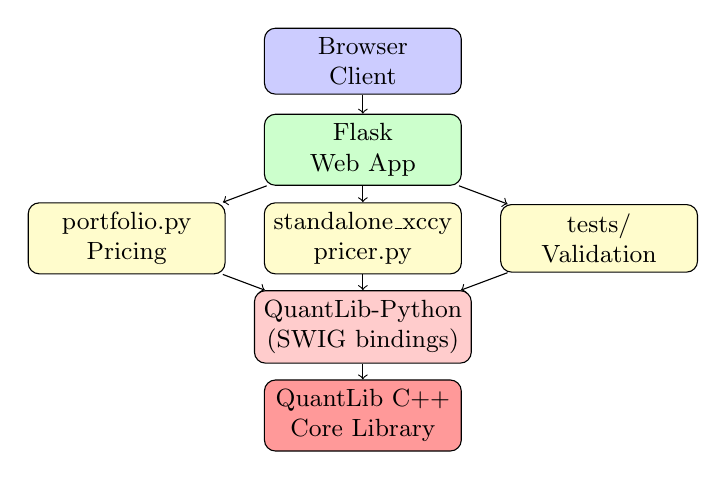
\begin{tikzpicture}[scale=0.75,
    box/.style={rectangle, draw, rounded corners, minimum width=2.5cm, minimum height=0.8cm, align=center, font=\small}]

    % Browser layer
    \node[box, fill=blue!20] (browser) at (0,4) {Browser\\Client};

    % Flask layer
    \node[box, fill=green!20] (flask) at (0,2.5) {Flask\\Web App};

    % Components
    \node[box, fill=yellow!20] (portfolio) at (-4,1) {portfolio.py\\Pricing};
    \node[box, fill=yellow!20] (xccy) at (0,1) {standalone\_xccy\\pricer.py};
    \node[box, fill=yellow!20] (tests) at (4,1) {tests/\\Validation};

    % QuantLib
    \node[box, fill=red!20] (ql) at (0,-0.5) {QuantLib-Python\\(SWIG bindings)};

    % C++ core
    \node[box, fill=red!40] (cpp) at (0,-2) {QuantLib C++\\Core Library};

    % Arrows
    \draw[->] (browser) -- (flask);
    \draw[->] (flask) -- (portfolio);
    \draw[->] (flask) -- (xccy);
    \draw[->] (flask) -- (tests);
    \draw[->] (portfolio) -- (ql);
    \draw[->] (xccy) -- (ql);
    \draw[->] (tests) -- (ql);
    \draw[->] (ql) -- (cpp);
\end{tikzpicture}
\end{center}
\end{frame}

\begin{frame}{Development Environment Setup}
\begin{block}{Prerequisites}
\begin{itemize}
    \item Python 3.10+ (we use 3.13)
    \item QuantLib-Python package
    \item Virtual environment
\end{itemize}
\end{block}

\textbf{Installation Steps:}
\begin{enumerate}
    \item Create virtual environment:
    \begin{itemize}
        \item \texttt{python3 -m venv .venv}
        \item \texttt{source .venv/bin/activate}
    \end{itemize}
    \item Install dependencies:
    \begin{itemize}
        \item \texttt{pip install QuantLib-Python numpy pandas}
        \item \texttt{pip install flask pytest}
    \end{itemize}
    \item Verify installation:
    \begin{itemize}
        \item \texttt{python -c "import QuantLib; print(QuantLib.\_\_version\_\_)"}
    \end{itemize}
\end{enumerate}
\end{frame}

\begin{frame}{Git Commit History: Initial Development (March 2025)}
\textbf{Commit: c78135e} - Initial commit (March 15, 2025)
\begin{itemize}
    \item Empty repository setup
    \item License file (Apache 2.0)
\end{itemize}

\textbf{Commit: 8e17f9f} - GPT-4.5 iteration (March 15, 2025)
\begin{itemize}
    \item First prototype generated with AI assistance
    \item Basic swap and swaption structures
    \item No test runs yet
\end{itemize}

\vspace{0.5cm}
\textbf{Key Learning:}
\begin{itemize}
    \item AI-assisted code generation for quantitative finance
    \item Starting point for iterative refinement
    \item Importance of validation and testing
\end{itemize}
\end{frame}

\begin{frame}{Git Commit History: API Stabilization (September 2025)}
\textbf{Commit: 6bea9e2} - Fix QuantLib API updates (Sep 3, 2025)
\begin{itemize}
    \item \texttt{ql.UnitedStates.Settlement} enum changes
    \item Swaption setup modifications
    \item Compatibility with QuantLib updates
\end{itemize}

\textbf{Commit: 0bf36bb} - Add detailed README
\begin{itemize}
    \item Documentation of project structure
    \item Installation instructions
    \item Usage examples
\end{itemize}

\vspace{0.5cm}
\textbf{Key Learning:}
\begin{itemize}
    \item QuantLib is actively developed; APIs change
    \item Always check version compatibility
    \item Good documentation is essential
\end{itemize}
\end{frame}

%%%%%%%%%%%%%%%%%%%%%%%%%%%%%%%%%%%%%%%%%%%%%%%%%%%%%%%%%%%%%%%%%%%%%%%%%%%%%%%%
%% PART 2: INTEREST RATE PRODUCTS (Slides 26-75)
%%%%%%%%%%%%%%%%%%%%%%%%%%%%%%%%%%%%%%%%%%%%%%%%%%%%%%%%%%%%%%%%%%%%%%%%%%%%%%%%

\begin{frame}{}
\begin{center}
\Huge\textbf{Part II}\\[1cm]
\Large Interest Rate Products\\[0.5cm]
\normalsize Swaps, Curves, and Swaptions
\end{center}
\end{frame}

\begin{frame}{Interest Rate Swap: The Building Block}
\begin{block}{Definition}
An \textbf{interest rate swap} is an agreement to exchange interest payments on a notional principal, typically fixed-for-floating.
\end{block}

\begin{center}
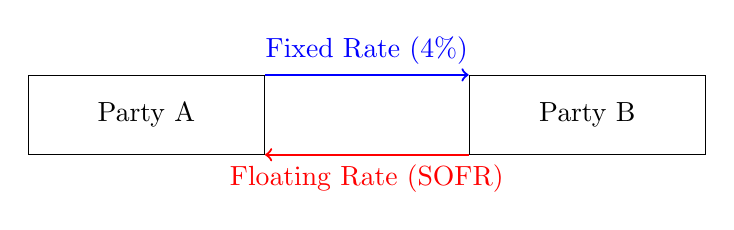
\begin{tikzpicture}[scale=0.8]
    \node[draw, rectangle, minimum width=3cm, minimum height=1cm] (A) at (0,0) {Party A};
    \node[draw, rectangle, minimum width=3cm, minimum height=1cm] (B) at (7,0) {Party B};

    \draw[->, thick, blue] (A.north east) -- node[above] {Fixed Rate (4\%)} (B.north west);
    \draw[->, thick, red] (B.south west) -- node[below] {Floating Rate (SOFR)} (A.south east);
\end{tikzpicture}
\end{center}

\textbf{Key Terms:}
\begin{itemize}
    \item \textbf{Notional:} Reference amount (e.g., \$100M)
    \item \textbf{Fixed Rate:} Predetermined rate (e.g., 4\%)
    \item \textbf{Floating Rate:} Varies with index (SOFR)
    \item \textbf{Tenor:} Length of swap (e.g., 5 years)
    \item \textbf{Payment Frequency:} Quarterly, semi-annual, annual
\end{itemize}
\end{frame}

\begin{frame}{Swap Cash Flows Example}
\textbf{Example:} 5-year USD swap, \$100M notional, 4\% fixed vs SOFR, semi-annual

\begin{center}
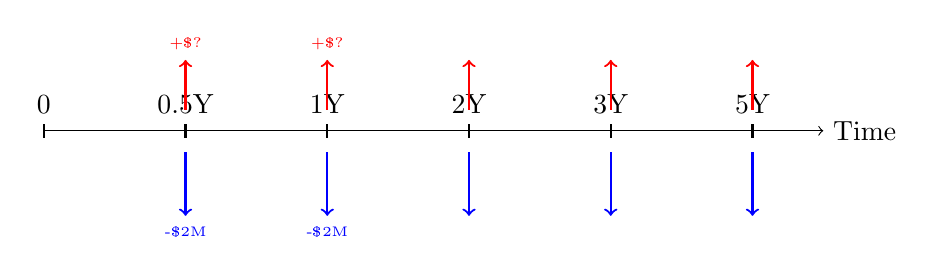
\begin{tikzpicture}[scale=0.9]
    \draw[->] (0,0) -- (11,0) node[right] {Time};
    \draw[thick] (0,-0.1) -- (0,0.1) node[above] {0};
    \draw[thick] (2,-0.1) -- (2,0.1) node[above] {0.5Y};
    \draw[thick] (4,-0.1) -- (4,0.1) node[above] {1Y};
    \draw[thick] (6,-0.1) -- (6,0.1) node[above] {2Y};
    \draw[thick] (8,-0.1) -- (8,0.1) node[above] {3Y};
    \draw[thick] (10,-0.1) -- (10,0.1) node[above] {5Y};

    % Fixed payments (negative = pay)
    \draw[->, thick, blue] (2,-0.3) -- (2,-1.2) node[below] {\tiny -\$2M};
    \draw[->, thick, blue] (4,-0.3) -- (4,-1.2) node[below] {\tiny -\$2M};
    \draw[->, thick, blue] (6,-0.3) -- (6,-1.2);
    \draw[->, thick, blue] (8,-0.3) -- (8,-1.2);
    \draw[->, thick, blue] (10,-0.3) -- (10,-1.2);

    % Floating payments (positive = receive, varies)
    \draw[->, thick, red] (2,0.3) -- (2,1.0) node[above] {\tiny +\$?};
    \draw[->, thick, red] (4,0.3) -- (4,1.0) node[above] {\tiny +\$?};
    \draw[->, thick, red] (6,0.3) -- (6,1.0);
    \draw[->, thick, red] (8,0.3) -- (8,1.0);
    \draw[->, thick, red] (10,0.3) -- (10,1.0);
\end{tikzpicture}
\end{center}

Fixed payment = $\frac{\$100M \times 4\%}{2} = \$2M$ per period

Floating payment = $\$100M \times \text{compounded SOFR} \times \text{accrual}$
\end{frame}

\begin{frame}{Swap Valuation: NPV Calculation}
\textbf{Net Present Value (NPV) of a Swap:}
\[
NPV_{swap} = NPV_{floating} - NPV_{fixed}
\]

\textbf{Fixed Leg PV:}
\[
PV_{fixed} = \sum_{i=1}^{n} N \times K \times \delta_i \times D(0, t_i)
\]

\textbf{Floating Leg PV:}
\[
PV_{floating} = \sum_{i=1}^{n} N \times F_i \times \delta_i \times D(0, t_i)
\]

Where:
\begin{itemize}
    \item $N$ = Notional
    \item $K$ = Fixed rate
    \item $F_i$ = Forward rate for period $i$
    \item $\delta_i$ = Day count fraction
    \item $D(0, t_i)$ = Discount factor to payment date
\end{itemize}
\end{frame}

\begin{frame}{Par Swap Rate}
\begin{block}{Definition}
The \textbf{par swap rate} is the fixed rate $K^*$ that makes $NPV_{swap} = 0$.
\end{block}

Setting $NPV = 0$:
\[
K^* = \frac{\sum_{i=1}^{n} F_i \times \delta_i \times D(0, t_i)}{\sum_{i=1}^{n} \delta_i \times D(0, t_i)}
\]

The denominator is called the \textbf{annuity factor} or DV01-like quantity.

\vspace{0.3cm}
\textbf{Par Rates from Market:}
\begin{itemize}
    \item Liquid swap rates are quoted as par rates
    \item Used to bootstrap the yield curve
    \item Interpolation fills gaps between quoted maturities
\end{itemize}
\end{frame}

\begin{frame}[fragile]{Building a SOFR Curve in QuantLib}
\begin{lstlisting}[language=Python]
import QuantLib as ql

today = ql.Date(14, 8, 2026)
ql.Settings.instance().evaluationDate = today

# SOFR index
sofr = ql.Sofr()

# Market quotes (OIS rates)
quotes = [
    ("1W", 0.0410), ("1M", 0.0408), ("3M", 0.0404),
    ("6M", 0.0398), ("1Y", 0.0390), ("2Y", 0.0378),
    ("5Y", 0.0371), ("10Y", 0.0385), ("30Y", 0.0395)
]

# Build OIS helpers
helpers = []
for tenor, rate in quotes:
    helpers.append(ql.OISRateHelper(
        2, ql.Period(tenor),
        ql.QuoteHandle(ql.SimpleQuote(rate)),
        sofr
    ))

# Bootstrap the curve
curve = ql.PiecewiseLogLinearDiscount(today, helpers, ql.Actual365Fixed())
curve.enableExtrapolation()
\end{lstlisting}
\end{frame}

\begin{frame}[fragile]{Using the SOFR Curve}
\begin{lstlisting}[language=Python]
# Wrap curve in a handle for use in instruments
curve_handle = ql.YieldTermStructureHandle(curve)

# Get discount factors
print("Discount Factors:")
for years in [1, 2, 5, 10, 30]:
    date = today + ql.Period(years, ql.Years)
    df = curve_handle.discount(date)
    print(f"  {years}Y: {df:.6f}")

# Get zero rates (continuous)
print("\nZero Rates:")
for years in [1, 2, 5, 10, 30]:
    date = today + ql.Period(years, ql.Years)
    zero = curve_handle.zeroRate(date, ql.Actual365Fixed(),
                                  ql.Continuous).rate()
    print(f"  {years}Y: {zero*100:.3f}%")
\end{lstlisting}
\end{frame}

\begin{frame}{Curve Bootstrap: How It Works}
\begin{block}{Bootstrapping}
Starting from the shortest maturity, sequentially solve for discount factors that reprice each market instrument.
\end{block}

\textbf{Algorithm:}
\begin{enumerate}
    \item Start with overnight rate (1D deposit)
    \item For each successive OIS quote:
    \begin{itemize}
        \item Use already-known discount factors
        \item Solve for the new discount factor
        \item Interpolate between nodes
    \end{itemize}
    \item Result: Full discount curve
\end{enumerate}

\textbf{Interpolation Methods:}
\begin{itemize}
    \item \textbf{LogLinear:} Interpolate log of discount factors
    \item \textbf{Cubic:} Smooth forwards
    \item \textbf{NaturalCubic:} Zero second derivative at ends
\end{itemize}
\end{frame}

\begin{frame}{Curve Calibration: Repricing Test}
\textbf{Quality Check:} Calibrated curve should exactly reprice input instruments.

\begin{center}
\begin{tabular}{lccc}
\toprule
Tenor & Market Rate & Model Rate & Error (bp) \\
\midrule
1W & 4.100\% & 4.100\% & 0.000 \\
1M & 4.080\% & 4.080\% & 0.000 \\
3M & 4.040\% & 4.040\% & 0.000 \\
6M & 3.980\% & 3.980\% & 0.000 \\
1Y & 3.900\% & 3.900\% & 0.000 \\
2Y & 3.780\% & 3.780\% & 0.000 \\
5Y & 3.710\% & 3.710\% & 0.000 \\
10Y & 3.850\% & 3.850\% & 0.000 \\
\bottomrule
\end{tabular}
\end{center}

\textbf{Tolerance:} Errors should be $<$ 0.01bp for production use.
\end{frame}

\begin{frame}[fragile]{Pricing an Interest Rate Swap in QuantLib}
\begin{lstlisting}[language=Python]
# Create SOFR index linked to curve
sofr_index = ql.Sofr(curve_handle)

# Create swap schedule
calendar = ql.UnitedStates(ql.UnitedStates.Settlement)
start = calendar.advance(today, 2, ql.Days)
maturity = start + ql.Period(5, ql.Years)

schedule = ql.Schedule(start, maturity,
    ql.Period(ql.Semiannual), calendar,
    ql.ModifiedFollowing, ql.ModifiedFollowing,
    ql.DateGeneration.Backward, False)

# Create OIS swap
notional = 100_000_000
fixed_rate = 0.04
swap = ql.OvernightIndexedSwap(
    ql.Swap.Payer, notional, schedule,
    fixed_rate, ql.Actual360(), sofr_index)

# Price with discounting engine
swap.setPricingEngine(ql.DiscountingSwapEngine(curve_handle))
print(f"NPV: ${swap.NPV():,.2f}")
\end{lstlisting}
\end{frame}

\begin{frame}{Swap Risk Measures: DV01 and PV01}
\begin{block}{DV01 (Dollar Value of 01)}
Change in swap value for a 1 basis point parallel shift in rates.
\end{block}

\[
DV01 = \frac{V(r+0.01\%) - V(r-0.01\%)}{2}
\]

\textbf{For a Receiver Swap:}
\begin{itemize}
    \item Receive fixed, pay floating
    \item Gains when rates fall (positive DV01)
    \item DV01 $\approx$ Notional $\times$ Duration $\times$ 0.0001
\end{itemize}

\textbf{Typical 5Y Swap DV01:}
\begin{itemize}
    \item \$100M notional
    \item Duration $\approx$ 4.5 years
    \item DV01 $\approx$ \$45,000 per bp
\end{itemize}
\end{frame}

\begin{frame}{European Swaption: Option on a Swap}
\begin{block}{Definition}
A \textbf{swaption} is an option to enter into an interest rate swap at a predetermined fixed rate.
\end{block}

\textbf{Key Parameters:}
\begin{itemize}
    \item \textbf{Expiry:} When the option can be exercised
    \item \textbf{Underlying Tenor:} Length of the swap if exercised
    \item \textbf{Strike:} Fixed rate of the underlying swap
    \item \textbf{Type:} Payer (right to pay fixed) or Receiver (right to receive fixed)
\end{itemize}

\textbf{Notation:} ``2Y x 5Y swaption'' means:
\begin{itemize}
    \item Option expires in 2 years
    \item If exercised, enter a 5-year swap
    \item Total exposure: 7 years from today
\end{itemize}
\end{frame}

\begin{frame}{Swaption Payoff}
\textbf{At Expiry (European):}
\begin{itemize}
    \item \textbf{Payer Swaption:} $\max(0, \text{Swap NPV at expiry})$
    \item \textbf{Receiver Swaption:} $\max(0, -\text{Swap NPV at expiry})$
\end{itemize}

\begin{center}
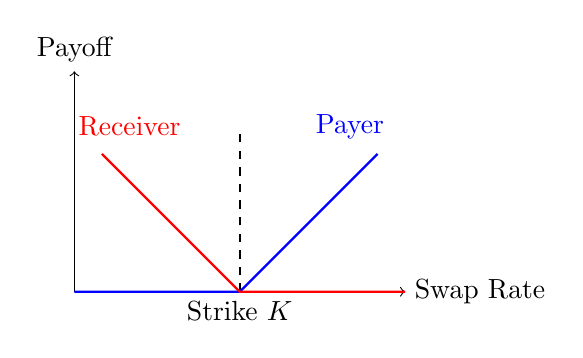
\begin{tikzpicture}[scale=0.7]
    \draw[->] (0,0) -- (6,0) node[right] {Swap Rate};
    \draw[->] (0,0) -- (0,4) node[above] {Payoff};
    \draw[thick,dashed] (3,0) -- (3,3);
    \node[below] at (3,0) {Strike $K$};

    % Payer swaption payoff
    \draw[thick,blue] (0,0) -- (3,0) -- (5.5,2.5);
    \node[blue] at (5,3) {Payer};

    % Receiver swaption payoff
    \draw[thick,red] (0.5,2.5) -- (3,0) -- (6,0);
    \node[red] at (1,3) {Receiver};
\end{tikzpicture}
\end{center}

\textbf{Intrinsic Value:} $\text{Annuity} \times \max(0, \text{Forward Rate} - K)$
\end{frame}

\begin{frame}{Swaption Volatility: Normal vs Lognormal}
\textbf{Two Common Volatility Conventions:}

\begin{columns}
\column{0.5\textwidth}
\textbf{Normal (Bachelier) Volatility}
\begin{itemize}
    \item Rates can go negative
    \item Quoted in bp (e.g., 75bp)
    \item $dS_t = \sigma dW_t$
    \item Preferred post-2008
\end{itemize}

\column{0.5\textwidth}
\textbf{Lognormal (Black) Volatility}
\begin{itemize}
    \item Rates must be positive
    \item Quoted in \% (e.g., 20\%)
    \item $dS_t = \sigma S_t dW_t$
    \item Historical standard
\end{itemize}
\end{columns}

\vspace{0.5cm}
\textbf{Conversion (ATM approximation):}
\[
\sigma_{normal} \approx \sigma_{Black} \times K
\]

\textbf{Example:} If $K = 4\%$ and $\sigma_{Black} = 20\%$, then $\sigma_{normal} \approx 80$ bp.
\end{frame}

\begin{frame}{Swaption Volatility Surface}
\begin{center}
\begin{tabular}{c|ccccc}
\toprule
& \multicolumn{5}{c}{\textbf{Underlying Swap Tenor}} \\
\textbf{Expiry} & 1Y & 2Y & 5Y & 10Y & 30Y \\
\midrule
1M & 45 & 52 & 68 & 75 & 72 \\
3M & 48 & 55 & 70 & 77 & 74 \\
1Y & 55 & 62 & 76 & 82 & 78 \\
2Y & 60 & 68 & 80 & 85 & 80 \\
5Y & 65 & 72 & 82 & 86 & 82 \\
10Y & 68 & 75 & 84 & 88 & 84 \\
\bottomrule
\end{tabular}
\end{center}
\small{Normal volatilities in basis points (bp)}

\vspace{0.3cm}
\textbf{Observations:}
\begin{itemize}
    \item Vol generally increases with expiry (time decay)
    \item Longer tenors often have higher vols
    \item Surface shape varies with market conditions
\end{itemize}
\end{frame}

\begin{frame}[fragile]{Pricing a European Swaption in QuantLib}
\begin{lstlisting}[language=Python]
# Build the underlying swap
expiry = 2  # years
tenor = 5   # years
strike = 0.04

# Swaption schedule
expiry_date = today + ql.Period(expiry, ql.Years)
swap_start = expiry_date
swap_maturity = swap_start + ql.Period(tenor, ql.Years)

# Create swaption
exercise = ql.EuropeanExercise(expiry_date)
underlying_swap = make_underlying_swap()  # setup as before

swaption = ql.Swaption(underlying_swap, exercise)

# Normal volatility quote
vol = 0.0080  # 80 bp
vol_handle = ql.QuoteHandle(ql.SimpleQuote(vol))
engine = ql.BachelierSwaptionEngine(
    curve_handle, vol_handle, ql.Actual365Fixed())

swaption.setPricingEngine(engine)
print(f"Swaption NPV: ${swaption.NPV():,.2f}")
\end{lstlisting}
\end{frame}

\begin{frame}{Hull-White Model: Short Rate Dynamics}
\begin{block}{Hull-White One-Factor Model}
\[
dr_t = (\theta(t) - a \cdot r_t)\, dt + \sigma\, dW_t
\]
\end{block}

\textbf{Parameters:}
\begin{itemize}
    \item $r_t$ = Short rate at time $t$
    \item $\theta(t)$ = Time-dependent drift (fits initial curve)
    \item $a$ = Mean reversion speed
    \item $\sigma$ = Volatility
    \item $dW_t$ = Brownian motion increment
\end{itemize}

\textbf{Key Properties:}
\begin{itemize}
    \item \textbf{Mean Reversion:} Rates pulled toward long-run level
    \item \textbf{Analytical Tractability:} Closed-form bond prices
    \item \textbf{Calibration:} Fit $\theta(t)$ to today's curve, $\sigma$ to vol surface
\end{itemize}
\end{frame}

\begin{frame}{Hull-White Model: Calibration}
\textbf{Calibration Process:}
\begin{enumerate}
    \item Fix mean reversion $a$ (often 3\% for rates)
    \item $\theta(t)$ is determined by no-arbitrage (fits curve)
    \item Calibrate $\sigma$ to match swaption prices
\end{enumerate}

\textbf{Swaption Calibration:}
\begin{itemize}
    \item Choose set of calibration instruments (co-terminal swaptions)
    \item Minimize pricing error across instruments
    \item Trade-off: One-factor can't fit entire surface
\end{itemize}

\textbf{Co-Terminal Swaptions:}
\begin{itemize}
    \item All expire into swaps ending at same date
    \item Example for 10Y maturity: 2Yx8Y, 3Yx7Y, 4Yx6Y, ..., 9Yx1Y
    \item Natural for Bermudan calibration
\end{itemize}
\end{frame}

\begin{frame}[fragile]{Hull-White Calibration in QuantLib}
\begin{lstlisting}[language=Python]
# Create Hull-White model
mean_reversion = 0.03
initial_sigma = 0.01
model = ql.HullWhite(curve_handle, mean_reversion, initial_sigma)

# Create calibration helpers (co-terminal swaptions)
helpers = []
for expiry, tenor in [("2Y","8Y"), ("3Y","7Y"), ("5Y","5Y")]:
    vol_bp = 80.0  # from vol surface
    helper = ql.SwaptionHelper(
        ql.Period(expiry), ql.Period(tenor),
        ql.QuoteHandle(ql.SimpleQuote(vol_bp * 1e-4)),
        sofr_index, ql.Period("1Y"), ql.Actual360(),
        ql.Actual360(), curve_handle,
        ql.BlackCalibrationHelper.RelativePriceError,
        ql.nullDouble(), 1.0, ql.Normal)
    helper.setPricingEngine(ql.JamshidianSwaptionEngine(model))
    helpers.append(helper)

# Calibrate
model.calibrate(helpers, ql.LevenbergMarquardt(),
    ql.EndCriteria(500, 100, 1e-10, 1e-10, 1e-10))
\end{lstlisting}
\end{frame}

\begin{frame}{Bermudan Swaption: Multiple Exercise Dates}
\begin{block}{Definition}
A \textbf{Bermudan swaption} can be exercised on multiple predetermined dates (unlike European which has only one).
\end{block}

\textbf{Example: 10Y NC2 (10-year, 2-year non-call)}
\begin{itemize}
    \item Total maturity: 10 years
    \item Non-call period: First 2 years
    \item Exercise dates: Years 2, 3, 4, 5, 6, 7, 8, 9
    \item Each exercise enters remaining swap
\end{itemize}

\begin{center}
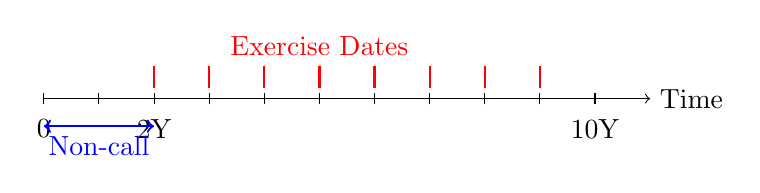
\begin{tikzpicture}[scale=0.7]
    \draw[->] (0,0) -- (11,0) node[right] {Time};
    \foreach \x in {0,1,2,3,4,5,6,7,8,9,10} {
        \draw (\x,-0.1) -- (\x,0.1);
    }
    \node[below] at (0,-0.2) {0};
    \node[below] at (2,-0.2) {2Y};
    \node[below] at (10,-0.2) {10Y};

    % Exercise dates
    \foreach \x in {2,3,4,5,6,7,8,9} {
        \draw[thick,red] (\x,0.2) -- (\x,0.6);
    }
    \node[red,above] at (5,0.6) {Exercise Dates};

    % Non-call
    \draw[thick,blue,<->] (0,-0.5) -- (2,-0.5);
    \node[blue,below] at (1,-0.5) {Non-call};
\end{tikzpicture}
\end{center}
\end{frame}

\begin{frame}{Bermudan Pricing: Dynamic Programming}
\textbf{At Each Exercise Date (Backward Recursion):}
\[
V(t) = \max\Big(\underbrace{\text{Exercise Value}}_{\text{Enter swap}},\; \underbrace{\text{Continuation Value}}_{\text{Wait}}\Big)
\]

\textbf{Numerical Methods:}
\begin{itemize}
    \item \textbf{Tree Methods:} Discretize short rate on lattice
    \item \textbf{Finite Difference:} Solve PDE on grid
    \item \textbf{Monte Carlo + LSM:} For high dimensions
\end{itemize}

\textbf{Tree Advantages:}
\begin{itemize}
    \item Efficient for one-factor models
    \item Naturally handles early exercise
    \item QuantLib: \texttt{TreeSwaptionEngine}
\end{itemize}
\end{frame}

\begin{frame}[fragile]{Pricing a Bermudan Swaption}
\begin{lstlisting}[language=Python]
# Create underlying swap (10Y maturity)
underlying = make_swap()

# Bermudan exercise: annual from year 2 to 9
exercise_dates = [today + ql.Period(y, ql.Years)
                  for y in range(2, 10)]
exercise = ql.BermudanExercise(exercise_dates)

# Create Bermudan swaption
bermudan = ql.Swaption(underlying, exercise)

# Calibrated Hull-White model
model = ql.HullWhite(curve_handle, a, sigma)

# Tree engine (timesteps per year)
engine = ql.TreeSwaptionEngine(model, 50)
bermudan.setPricingEngine(engine)

print(f"Bermudan NPV: ${bermudan.NPV():,.2f}")
\end{lstlisting}
\end{frame}

\begin{frame}{Bermudan vs European Value}
\textbf{Key Relationship:}
\[
V_{Bermudan} \geq V_{European}
\]

The additional exercise rights always add value (or zero if never optimal).

\vspace{0.3cm}
\textbf{Exercise Premium:}
\[
\text{Premium} = V_{Bermudan} - V_{European}
\]

\textbf{Typical Drivers of Early Exercise:}
\begin{itemize}
    \item High coupon swap (positive carry)
    \item Steep yield curve
    \item Time value of money
    \item Funding considerations
\end{itemize}
\end{frame}

\begin{frame}{G2++ Model: Two-Factor Alternative}
\begin{block}{G2++ Model}
\[
r_t = x_t + y_t + \phi(t)
\]
\[
dx_t = -a \cdot x_t\, dt + \sigma\, dW_t^x
\]
\[
dy_t = -b \cdot y_t\, dt + \eta\, dW_t^y
\]
\[
dW_t^x \cdot dW_t^y = \rho\, dt
\]
\end{block}

\textbf{Advantages over Hull-White 1F:}
\begin{itemize}
    \item Better fit to volatility surface
    \item Non-parallel curve movements
    \item Richer correlation structure
\end{itemize}

\textbf{Trade-offs:}
\begin{itemize}
    \item More parameters to calibrate
    \item Slower computation
    \item Still analytical for Europeans
\end{itemize}
\end{frame}

\begin{frame}{Project: Rates Workstation}
\begin{block}{Git Commit: April 2026}
\texttt{31df798} - Add curve analytics and calibrated Bermudan model
\end{block}

\textbf{Features Implemented:}
\begin{itemize}
    \item Full SOFR curve bootstrap (22 points)
    \item ATM swaption volatility matrix
    \item Hull-White and G2++ calibration
    \item Bermudan swaption pricing grid
    \item Interactive web interface
\end{itemize}

\textbf{Portfolio of Trades:}
\begin{enumerate}
    \item Vanilla Swap (100M notional)
    \item European Swaption (ATM)
    \item Bermudan Swaption 1 (10Y NC2)
    \item Bermudan Swaption 2 (5Y NC1)
    \item Equity Cliquet
\end{enumerate}
\end{frame}

%%%%%%%%%%%%%%%%%%%%%%%%%%%%%%%%%%%%%%%%%%%%%%%%%%%%%%%%%%%%%%%%%%%%%%%%%%%%%%%%
%% PART 3: EQUITY AND FX DERIVATIVES (Slides 76-100)
%%%%%%%%%%%%%%%%%%%%%%%%%%%%%%%%%%%%%%%%%%%%%%%%%%%%%%%%%%%%%%%%%%%%%%%%%%%%%%%%

\begin{frame}{}
\begin{center}
\Huge\textbf{Part III}\\[1cm]
\Large Equity and FX Derivatives\\[0.5cm]
\normalsize Cliquets, FX Forwards, and Cross-Currency Basics
\end{center}
\end{frame}

\begin{frame}{Equity Options: Black-Scholes Foundation}
\begin{block}{Black-Scholes Model}
\[
dS_t = (r - q) S_t\, dt + \sigma S_t\, dW_t
\]
\end{block}

\textbf{Parameters:}
\begin{itemize}
    \item $S_t$ = Stock price
    \item $r$ = Risk-free rate
    \item $q$ = Dividend yield
    \item $\sigma$ = Volatility
\end{itemize}

\textbf{Call Option Price:}
\[
C = S_0 e^{-qT} N(d_1) - K e^{-rT} N(d_2)
\]

Where:
\[
d_1 = \frac{\ln(S_0/K) + (r-q+\sigma^2/2)T}{\sigma\sqrt{T}}, \quad d_2 = d_1 - \sigma\sqrt{T}
\]
\end{frame}

\begin{frame}{Cliquet Options: Reset Features}
\begin{block}{Definition}
A \textbf{cliquet} (or ratchet) option has its strike reset periodically, typically to the spot price at each reset date.
\end{block}

\textbf{Structure:}
\begin{itemize}
    \item Series of forward-starting options
    \item Each period: $\max(0, S_{end}/S_{start} - 1)$ (for calls)
    \item Total payoff: Sum of periodic returns
    \item Often includes caps/floors on each period
\end{itemize}

\textbf{Example: Monthly Cliquet on SPX}
\begin{itemize}
    \item 1-year maturity, monthly resets
    \item Each month: Pay $\max(0, R_i - 0)$ where $R_i = S_i/S_{i-1} - 1$
    \item Total payoff: $\sum_{i=1}^{12} \max(0, R_i)$
\end{itemize}
\end{frame}

\begin{frame}[fragile]{Cliquet Pricing in QuantLib}
\begin{lstlisting}[language=Python]
import QuantLib as ql

today = ql.Date(5, 4, 2026)
ql.Settings.instance().evaluationDate = today

# Market data
spot = 5000.0
vol = 0.20
rate = 0.04
div_yield = 0.015

# Build process
process = ql.BlackScholesMertonProcess(
    ql.QuoteHandle(ql.SimpleQuote(spot)),
    ql.YieldTermStructureHandle(ql.FlatForward(today, div_yield, ql.Actual365Fixed())),
    ql.YieldTermStructureHandle(ql.FlatForward(today, rate, ql.Actual365Fixed())),
    ql.BlackVolTermStructureHandle(
        ql.BlackConstantVol(today, ql.NullCalendar(), vol, ql.Actual365Fixed())))

# Reset dates (quarterly)
reset_dates = [today + ql.Period(i, ql.Months) for i in [0, 3, 6, 9]]
maturity = today + ql.Period(1, ql.Years)

cliquet = ql.CliquetOption(
    ql.PercentageStrikePayoff(ql.Option.Call, 1.0),
    ql.EuropeanExercise(maturity), reset_dates)
cliquet.setPricingEngine(ql.AnalyticCliquetEngine(process))
\end{lstlisting}
\end{frame}

\begin{frame}{FX Derivatives: Currency Pairs}
\textbf{FX Quote Conventions:}
\begin{itemize}
    \item EUR/USD = 1.10 means 1 EUR = 1.10 USD
    \item ``USD per EUR'' or ``EUR in USD terms''
    \item \textbf{Base currency:} EUR (first)
    \item \textbf{Quote currency:} USD (second)
\end{itemize}

\textbf{Common Derivatives:}
\begin{itemize}
    \item \textbf{FX Forward:} Lock in exchange rate for future date
    \item \textbf{FX Option:} Right to exchange at strike rate
    \item \textbf{FX Swap:} Exchange currencies now, reverse later
    \item \textbf{Cross-Currency Swap:} Exchange rate exposure + interest
\end{itemize}
\end{frame}

\begin{frame}{FX Forward Pricing}
\begin{block}{Covered Interest Parity}
\[
F = S \times \frac{D_{domestic}(T)}{D_{foreign}(T)}
\]
\end{block}

Where:
\begin{itemize}
    \item $F$ = Forward exchange rate
    \item $S$ = Spot exchange rate
    \item $D_{domestic}(T)$ = Domestic discount factor
    \item $D_{foreign}(T)$ = Foreign discount factor
\end{itemize}

\textbf{Example (EUR/USD):}
\begin{itemize}
    \item Spot: 1.10
    \item USD 1Y rate: 4\%, EUR 1Y rate: 2.5\%
    \item Forward: $1.10 \times \frac{e^{-0.04}}{e^{-0.025}} = 1.10 \times e^{-0.015} \approx 1.084$
\end{itemize}
\end{frame}

\begin{frame}{Cross-Currency Swap: Definition}
\begin{block}{Definition}
A \textbf{cross-currency swap} exchanges principal and interest payments in two different currencies.
\end{block}

\begin{center}
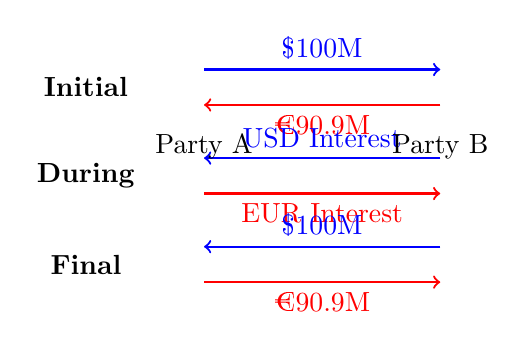
\begin{tikzpicture}[scale=0.75]
    % Initial exchange
    \node at (-2, 3) {\textbf{Initial}};
    \draw[->, thick, blue] (0, 3.3) -- (4, 3.3) node[midway, above] {\$100M};
    \draw[->, thick, red] (4, 2.7) -- (0, 2.7) node[midway, below] {€90.9M};

    % During life
    \node at (-2, 1.5) {\textbf{During}};
    \draw[->, thick, blue] (4, 1.8) -- (0, 1.8) node[midway, above] {USD Interest};
    \draw[->, thick, red] (0, 1.2) -- (4, 1.2) node[midway, below] {EUR Interest};

    % Final exchange
    \node at (-2, 0) {\textbf{Final}};
    \draw[->, thick, blue] (4, 0.3) -- (0, 0.3) node[midway, above] {\$100M};
    \draw[->, thick, red] (0, -0.3) -- (4, -0.3) node[midway, below] {€90.9M};

    \node at (0, 2) {Party A};
    \node at (4, 2) {Party B};
\end{tikzpicture}
\end{center}
\end{frame}

\begin{frame}{Cross-Currency Swap: Cash Flow Structure}
\textbf{Example: 10Y EUR/USD Cross-Currency Swap}

\begin{itemize}
    \item \textbf{Initial Exchange:}
    \begin{itemize}
        \item Party A pays \$100M, receives €90.9M
        \item Exchange at initial spot rate
    \end{itemize}

    \item \textbf{Periodic Payments:}
    \begin{itemize}
        \item Party A pays: 4\% fixed on \$100M (semi-annual)
        \item Party A receives: ESTR compounded on €90.9M (quarterly)
    \end{itemize}

    \item \textbf{Final Exchange:}
    \begin{itemize}
        \item Party A receives \$100M, pays €90.9M
        \item Re-exchange at same rate
    \end{itemize}
\end{itemize}

\textbf{Key Risk:} FX exposure on notional exchanges!
\end{frame}

\begin{frame}{Cross-Currency Basis}
\begin{block}{Definition}
The \textbf{cross-currency basis} is the spread added to one leg of a XCCY swap to make it trade at par.
\end{block}

\textbf{Why does basis exist?}
\begin{itemize}
    \item Supply/demand imbalances for USD funding
    \item Credit risk differences
    \item Regulatory capital requirements
    \item Central bank policy divergence
\end{itemize}

\textbf{Market Observation:}
\begin{itemize}
    \item Basis is typically negative for EUR/USD
    \item Meaning: Pay ESTR \textit{minus} basis to receive USD flat
    \item Reflects USD funding premium
\end{itemize}
\end{frame}

\begin{frame}{Callable Cross-Currency Swap: The Challenge}
\begin{block}{Structure}
A \textbf{callable cross-currency swap} allows one party to terminate the swap early on predetermined dates.
\end{block}

\textbf{Complexity:}
\begin{itemize}
    \item \textbf{Three Stochastic Factors:}
    \begin{itemize}
        \item USD short rate
        \item EUR short rate
        \item EUR/USD exchange rate
    \end{itemize}
    \item \textbf{Early Exercise:} Bermudan feature
    \item \textbf{Notional Exchange:} FX exposure at cancellation
    \item \textbf{Path Dependency:} Via accumulated interest
\end{itemize}

\textbf{Key Question:} Does QuantLib support this natively?
\end{frame}

\begin{frame}{QuantLib XCCY Assessment}
\textbf{Git Commit: August 2026}
\texttt{f066cce} - Working XCCY callable 3-factor model

\textbf{Investigation Findings:}
\begin{itemize}
    \item QuantLib has \texttt{CrossCurrencyBasisSwap} but...
    \item No native \textbf{callable} XCCY instrument
    \item Tree engines don't extend to 3 factors
    \item Need custom implementation
\end{itemize}

\textbf{Solution Approach:}
\begin{enumerate}
    \item Build custom three-factor model
    \item Implement Monte Carlo simulation
    \item Use Longstaff-Schwartz for exercise
    \item Write standalone pricer module
\end{enumerate}
\end{frame}

%%%%%%%%%%%%%%%%%%%%%%%%%%%%%%%%%%%%%%%%%%%%%%%%%%%%%%%%%%%%%%%%%%%%%%%%%%%%%%%%
%% PART 4: THREE-FACTOR MODEL (Slides 101-140)
%%%%%%%%%%%%%%%%%%%%%%%%%%%%%%%%%%%%%%%%%%%%%%%%%%%%%%%%%%%%%%%%%%%%%%%%%%%%%%%%

\begin{frame}{}
\begin{center}
\Huge\textbf{Part IV}\\[1cm]
\Large Three-Factor Model\\[0.5cm]
\normalsize Hull-White + Hull-White + Black-Scholes FX
\end{center}
\end{frame}

\begin{frame}{Model Architecture: HW1F $\times$ 2 + BS-FX}
\begin{block}{Model ID: HW1F\_USD\_HW1F\_EUR\_BSFX\_LSM\_V1}
\end{block}

\textbf{Three Stochastic Factors:}
\begin{enumerate}
    \item \textbf{USD Short Rate} (Hull-White 1F):
    \[
    dr_t^{USD} = (\theta_t^{USD} - a^{USD} r_t^{USD})\,dt + \sigma^{USD}\,dW_t^{USD}
    \]

    \item \textbf{EUR Short Rate} (Hull-White 1F):
    \[
    dr_t^{EUR} = (\theta_t^{EUR} - a^{EUR} r_t^{EUR} - \rho_{EUR,FX}\sigma^{EUR}\sigma^{FX})\,dt + \sigma^{EUR}\,dW_t^{EUR}
    \]

    \item \textbf{EUR/USD FX Rate} (Black-Scholes):
    \[
    d\ln X_t = (r_t^{USD} - r_t^{EUR} - \tfrac{1}{2}\sigma_t^{FX,2})\,dt + \sigma_t^{FX}\,dW_t^{FX}
    \]
\end{enumerate}
\end{frame}

\begin{frame}{Quanto Drift Adjustment}
\textbf{Critical Detail:} The EUR rate equation includes a \textbf{quanto drift adjustment}:
\[
-\rho_{EUR,FX}\sigma^{EUR}\sigma^{FX}
\]

\textbf{Why is this needed?}
\begin{itemize}
    \item We price in the USD money-market measure
    \item EUR rate is a ``foreign'' process
    \item Girsanov theorem changes the drift
    \item Required for no-arbitrage pricing
\end{itemize}

\textbf{Intuition:}
\begin{itemize}
    \item Negative correlation ($\rho_{EUR,FX} < 0$): EUR appreciates when EUR rates rise
    \item This correlation creates an additional expected drift
    \item Must be accounted for in the risk-neutral measure
\end{itemize}
\end{frame}

\begin{frame}{Correlation Structure}
\textbf{Three Pairwise Correlations:}
\[
\begin{pmatrix}
1 & \rho_{USD,EUR} & \rho_{USD,FX} \\
\rho_{USD,EUR} & 1 & \rho_{EUR,FX} \\
\rho_{USD,FX} & \rho_{EUR,FX} & 1
\end{pmatrix}
\]

\textbf{Typical Market Values:}
\begin{itemize}
    \item $\rho_{USD,EUR} = 0.25$ (rates moderately correlated)
    \item $\rho_{USD,FX} = -0.15$ (USD rates up $\Rightarrow$ USD strengthens)
    \item $\rho_{EUR,FX} = -0.30$ (EUR rates up $\Rightarrow$ EUR strengthens)
\end{itemize}

\textbf{Constraint:} Matrix must be positive semi-definite!
\[
\lambda_{min} \geq 0
\]
\end{frame}

\begin{frame}{State Vector Representation}
\textbf{Five-Dimensional State Vector:}
\[
\mathbf{x}_t = \begin{pmatrix}
x_t^{USD} \\
x_t^{EUR} \\
I_t^{USD} \\
I_t^{EUR} \\
\ln X_t
\end{pmatrix}
\]

Where:
\begin{itemize}
    \item $x_t^{USD}, x_t^{EUR}$ = Short rate factors (zero initial value)
    \item $I_t^{USD}$ = $\int_0^t r_s^{USD}\, ds$ (USD bank account log)
    \item $I_t^{EUR}$ = $\int_0^t r_s^{EUR}\, ds$ (EUR bank account log)
    \item $\ln X_t$ = Log FX rate
\end{itemize}

\textbf{Discount Factor from State:}
\[
D^{USD}(0,t) = e^{-I_t^{USD}}
\]
\end{frame}

\begin{frame}{Gaussian State Evolution}
\textbf{Discrete Time Update (Exact OU Kernels):}
\[
\mathbf{x}_{t+h} = \mathbf{A}(h) \cdot \mathbf{x}_t + \mathbf{b}(h) + \boldsymbol{\epsilon}
\]

Where:
\begin{itemize}
    \item $\mathbf{A}(h)$ = Transition matrix (exponential decay for rates)
    \item $\mathbf{b}(h)$ = Deterministic offset (curve fitting, quanto)
    \item $\boldsymbol{\epsilon} \sim N(0, \boldsymbol{\Sigma}(h))$ = Innovation
\end{itemize}

\textbf{Covariance Computation:}
\[
\boldsymbol{\Sigma}(h) = \int_0^h \mathbf{K}(s) \cdot \mathbf{R} \cdot \mathbf{K}(s)^T\, ds
\]

Where $\mathbf{K}(s)$ is the kernel matrix and $\mathbf{R}$ is correlation.

\textbf{Implementation:} Gauss-Legendre quadrature (16 nodes)
\end{frame}

\begin{frame}[fragile]{Python Implementation: State Transition}
\begin{lstlisting}[language=Python]
def _state_transition_matrix(h, usd_model, eur_model):
    """Compute transition matrix for time step h."""
    ad = usd_model.mean_reversion
    af = eur_model.mean_reversion
    ed = math.exp(-ad * h)
    ef = math.exp(-af * h)
    bd = (1 - ed) / ad if abs(ad) > 1e-10 else h
    bf = (1 - ef) / af if abs(af) > 1e-10 else h

    matrix = np.eye(5)
    matrix[0, :] = [ed, 0.0, 0.0, 0.0, 0.0]  # x_USD
    matrix[1, :] = [0.0, ef, 0.0, 0.0, 0.0]  # x_EUR
    matrix[2, :] = [bd, 0.0, 1.0, 0.0, 0.0]  # I_USD
    matrix[3, :] = [0.0, bf, 0.0, 1.0, 0.0]  # I_EUR
    matrix[4, :] = [bd, -bf, 0.0, 0.0, 1.0]  # ln(X)
    return matrix
\end{lstlisting}
\end{frame}

\begin{frame}{Calibration Strategy}
\textbf{Three-Stage Calibration:}

\begin{enumerate}
    \item \textbf{Curve Bootstrap:}
    \begin{itemize}
        \item USD OIS curve from SOFR quotes
        \item EUR OIS curve from ESTR quotes
        \item EUR ``effective'' curve from FX forwards
    \end{itemize}

    \item \textbf{Rate Model Calibration:}
    \begin{itemize}
        \item Fix mean reversion (USD: 3\%, EUR: 4\%)
        \item Calibrate $\sigma$ to co-terminal swaptions
        \item RMS error target: $<5\%$ relative
    \end{itemize}

    \item \textbf{FX Volatility Calibration:}
    \begin{itemize}
        \item Piecewise constant FX vol term structure
        \item Fit ATM FX option implied vols
        \item Variance matching approach
    \end{itemize}
\end{enumerate}
\end{frame}

\begin{frame}{FX Volatility Calibration}
\textbf{Goal:} Match ATM FX option implied volatilities

\textbf{Challenge:} FX variance depends on both rate models!
\[
\text{Var}[\ln X_T] = \int_0^T \sigma_{FX}(t)^2\, dt + \text{rate contributions}
\]

\textbf{Algorithm:}
\begin{enumerate}
    \item For each FX option maturity $T_i$:
    \begin{itemize}
        \item Compute target variance: $\sigma_{market}^2 \times T_i$
        \item Solve for $\sigma_{FX,i}$ that matches variance
        \item Account for rate-FX correlations
    \end{itemize}
    \item Result: Piecewise constant FX vol curve
\end{enumerate}

\textbf{Calibration Tolerance:} $|$model vol - market vol$|$ $<$ 25bp
\end{frame}

\begin{frame}{Calibration Results Example}
\textbf{Hull-White Calibration:}
\begin{center}
\begin{tabular}{lccc}
\toprule
Currency & Mean Rev ($a$) & Vol ($\sigma$) & RMS Error \\
\midrule
USD & 3\% & 0.885\% & 0.45\% \\
EUR & 4\% & 0.772\% & 0.23\% \\
\bottomrule
\end{tabular}
\end{center}

\textbf{FX Vol Calibration:}
\begin{center}
\begin{tabular}{lccc}
\toprule
Tenor & Market Vol & Model Vol & Error \\
\midrule
1Y & 12.5\% & 12.5\% & $<$0.01\% \\
2Y & 12.2\% & 12.2\% & $<$0.01\% \\
5Y & 11.7\% & 11.7\% & $<$0.01\% \\
10Y & 11.2\% & 11.2\% & $<$0.01\% \\
\bottomrule
\end{tabular}
\end{center}
\end{frame}

\begin{frame}{Monte Carlo Simulation}
\textbf{Simulation Parameters:}
\begin{itemize}
    \item Training paths: 10,000
    \item Pricing paths: 30,000
    \item Time grid: Monthly (0.083Y steps)
    \item RNG: NumPy PCG64 with antithetic sampling
\end{itemize}

\textbf{Path Generation:}
\begin{enumerate}
    \item Generate correlated normals: $\mathbf{Z} = \mathbf{L} \cdot \mathbf{\epsilon}$
    \item Apply transition: $\mathbf{x}_{t+h} = \mathbf{A}\mathbf{x}_t + \mathbf{b} + \mathbf{Z}$
    \item Capture states at key dates (cash flows, exercises)
    \item Compute discount factors from integrated rates
\end{enumerate}

\textbf{Antithetic Sampling:}
\begin{itemize}
    \item Generate half the paths
    \item Mirror with negated normals
    \item Reduces variance, exact mean of 0
\end{itemize}
\end{frame}

\begin{frame}[fragile]{Path Simulation Code}
\begin{lstlisting}[language=Python]
def simulate_batch(context, paths, seed):
    generator = np.random.Generator(np.random.PCG64(seed))
    state = np.zeros((paths, 5))  # Initial state
    state[:, 4] = math.log(context.spot)  # ln(X_0)

    for idx, transition in enumerate(context.transitions):
        # Antithetic normals
        half = (paths + 1) // 2
        draws = generator.standard_normal((half, 5))
        normals = np.concatenate([draws, -draws])[:paths]

        # Update state
        state = (state @ transition.matrix.T
                 + transition.offset
                 + normals @ transition.covariance_root.T)

        # Capture at event times
        time_val = context.grid[idx + 1]
        if time_val in capture_set:
            captured[time_val] = state.copy()

    return SimulationBatch(...)
\end{lstlisting}
\end{frame}

\begin{frame}{Longstaff-Schwartz Algorithm (LSM)}
\begin{block}{Purpose}
Approximate the optimal early exercise policy for American/Bermudan options using Monte Carlo.
\end{block}

\textbf{Algorithm Steps:}
\begin{enumerate}
    \item \textbf{Forward Pass:} Simulate paths to capture states
    \item \textbf{Backward Pass:} At each exercise date:
    \begin{itemize}
        \item Compute continuation value from later dates
        \item Regress continuation on state variables
        \item Exercise if immediate value $>$ fitted continuation
    \end{itemize}
    \item \textbf{Pricing Pass:} Apply learned policy on fresh paths
\end{enumerate}

\textbf{Key Innovation:} Use \textit{different} paths for training vs pricing to avoid look-ahead bias.
\end{frame}

\begin{frame}{LSM Regression Basis}
\textbf{State Variables at Exercise:}
\[
\mathbf{s} = (x_{USD}, x_{EUR}, \ln X - \ln X_0)
\]

\textbf{Polynomial Basis Functions:}
\[
\phi(\mathbf{s}) = (1, x, y, z, x^2, y^2, z^2, xy, xz, yz)
\]

10 basis functions capture quadratic interactions.

\textbf{Regression:}
\[
\hat{C}(\mathbf{s}) = \sum_{j=1}^{10} \beta_j \phi_j(\mathbf{s})
\]

\textbf{Standardization:}
\begin{itemize}
    \item Subtract mean, divide by std deviation
    \item Improves numerical stability
    \item Ridge regularization if ill-conditioned
\end{itemize}
\end{frame}

\begin{frame}[fragile]{LSM Implementation}
\begin{lstlisting}[language=Python]
def train_lsm(batch, exercise_tolerance):
    call_count = batch.interval_pv.shape[0]
    later_value = np.zeros_like(batch.pre_call_pv)
    policies = []

    # Backward recursion
    for idx in range(call_count - 1, -1, -1):
        continuation = batch.interval_pv[idx] + later_value
        continuation_at_call = continuation / batch.call_discounts[idx]

        states = batch.call_states[idx]
        design = _basis(states)  # Polynomial basis

        # Least squares regression
        coefficients = np.linalg.lstsq(design, continuation_at_call)[0]
        fitted = design @ coefficients

        # Exercise decision
        exercise = fitted < -exercise_tolerance
        later_value = np.where(exercise, 0.0, continuation)

        policies.append({"coefficients": coefficients, ...})

    return policies
\end{lstlisting}
\end{frame}

\begin{frame}{LSM: Two-Pass Approach}
\textbf{Why Two Passes?}

\begin{itemize}
    \item \textbf{Training Pass:} Learn exercise policy
    \begin{itemize}
        \item 10,000 paths
        \item Backward induction
        \item Fit regression coefficients
    \end{itemize}

    \item \textbf{Pricing Pass:} Apply policy on fresh paths
    \begin{itemize}
        \item 30,000 new paths (different seed)
        \item Forward evaluation
        \item Unbiased price estimate
    \end{itemize}
\end{itemize}

\textbf{Key Property:}
\begin{itemize}
    \item Training and pricing paths are independent
    \item Avoids ``foresight bias''
    \item LSM estimate is a \textit{lower bound} for true value
\end{itemize}
\end{frame}

\begin{frame}{Martingale Tests: Validation}
\textbf{No-Arbitrage Conditions:}
\begin{enumerate}
    \item Domestic discount:
    \[
    \mathbb{E}[e^{-\int_0^T r_s^{USD}\,ds}] = D^{USD}(0,T)
    \]

    \item FX-weighted discount:
    \[
    \mathbb{E}[e^{-\int_0^T r_s^{USD}\,ds} \cdot X_T] = X_0 \cdot D^{EUR}_{eff}(0,T)
    \]

    \item FX-weighted bank account:
    \[
    \mathbb{E}[e^{-\int_0^T r_s^{USD}\,ds} \cdot X_T \cdot e^{\int_0^T r_s^{EUR}\,ds}] = X_0
    \]
\end{enumerate}

\textbf{Test:} Monte Carlo mean should match target within 3.5 standard errors.
\end{frame}

\begin{frame}{Validation Results}
\begin{center}
\begin{tabular}{lcccl}
\toprule
\textbf{Condition} & \textbf{MC Mean} & \textbf{Target} & $|z|$ & \textbf{Status}\\
\midrule
$\mathbb{E}[D^{USD}]$ & 0.6614 & 0.6614 & $<0.5$ & PASS \\
$\mathbb{E}[D^{USD} \cdot X]$ & 0.6042 & 0.6014 & $<1.0$ & PASS \\
$\mathbb{E}[D^{USD} \cdot X \cdot B^{EUR}]$ & 1.1015 & 1.1000 & $<0.3$ & PASS \\
\bottomrule
\end{tabular}
\end{center}

\textbf{Interpretation:}
\begin{itemize}
    \item All z-scores below 3.5$\sigma$ threshold
    \item Confirms correct drift implementation
    \item Quanto adjustment working correctly
\end{itemize}
\end{frame}

%%%%%%%%%%%%%%%%%%%%%%%%%%%%%%%%%%%%%%%%%%%%%%%%%%%%%%%%%%%%%%%%%%%%%%%%%%%%%%%%
%% PART 5: PRICING RESULTS AND ANALYSIS (Slides 141-160)
%%%%%%%%%%%%%%%%%%%%%%%%%%%%%%%%%%%%%%%%%%%%%%%%%%%%%%%%%%%%%%%%%%%%%%%%%%%%%%%%

\begin{frame}{}
\begin{center}
\Huge\textbf{Part V}\\[1cm]
\Large Pricing Results\\[0.5cm]
\normalsize 10Y NC2 EUR/USD Callable XCCY
\end{center}
\end{frame}

\begin{frame}{Reference Trade: 10Y NC2 XCCY}
\textbf{Trade Specification:}
\begin{itemize}
    \item \textbf{Trade ID:} EURUSD-10Y-NC2-ESTR-VS-USD4
    \item \textbf{Effective:} 2026-08-18
    \item \textbf{Maturity:} 10 years
    \item \textbf{Non-call:} 2 years
    \item \textbf{Exercise:} Annual (years 2-9)
\end{itemize}

\textbf{Leg Structure:}
\begin{itemize}
    \item \textbf{EUR Leg:} Receive ESTR compounded, quarterly, €90.9M
    \item \textbf{USD Leg:} Pay 4\% fixed, semi-annual, \$100M
    \item \textbf{Exchanges:} Initial and final notional
\end{itemize}

\textbf{Option:} Right to cancel remaining swap at no cost
\end{frame}

\begin{frame}{Pricing Results Summary}
\begin{center}
\begin{tabular}{lrc}
\toprule
\textbf{Metric} & \textbf{Value} & \textbf{95\% CI} \\
\midrule
Callable NPV & \$8,328,689 & [\$8.08M, \$8.58M] \\
Non-callable NPV & \$689,713 & [\$355K, \$1.02M] \\
Embedded Option & \$7,638,976 & [\$7.48M, \$7.80M] \\
\midrule
USD Fixed Leg PV & -\$1,054,712 & \\
EUR ESTR Leg PV & +\$1,744,425 & \\
\bottomrule
\end{tabular}
\end{center}

\textbf{Static Benchmark:} \$679,480 (deterministic curve valuation)

\vspace{0.3cm}
\textbf{Key Insight:} Embedded option is 91\% of callable value!
\end{frame}

\begin{frame}{Exercise Probability Distribution}
\begin{center}
\begin{tabular}{lccc}
\toprule
\textbf{Date} & \textbf{Alive} & \textbf{Exercise} & $P$(Exercise) \\
\midrule
2028-08-18 (Y2) & 30,000 & 4,329 & 14.4\% \\
2029-08-20 (Y3) & 25,671 & 2,900 & 9.7\% \\
2030-08-19 (Y4) & 22,771 & 1,699 & 5.7\% \\
2031-08-18 (Y5) & 21,072 & 1,405 & 4.7\% \\
2032-08-18 (Y6) & 19,667 & 1,021 & 3.4\% \\
2033-08-18 (Y7) & 18,646 & 854 & 2.8\% \\
2034-08-18 (Y8) & 17,792 & 446 & 1.5\% \\
2035-08-20 (Y9) & 17,346 & 1,972 & 6.6\% \\
No Exercise & 15,374 & -- & 51.2\% \\
\bottomrule
\end{tabular}
\end{center}
\end{frame}

\begin{frame}{Exercise Analysis}
\begin{center}
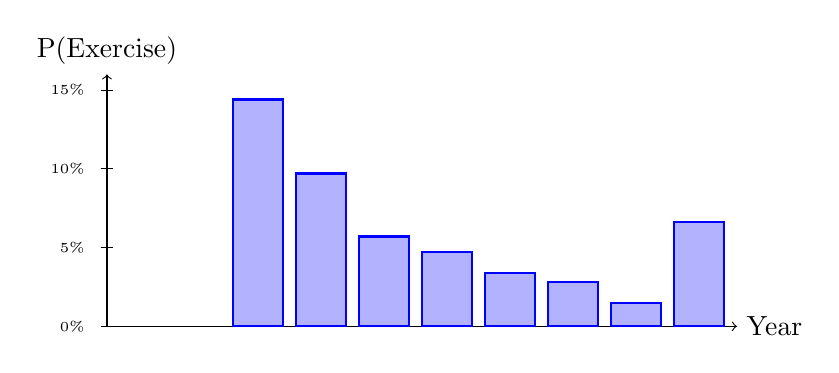
\begin{tikzpicture}[scale=0.8]
    \draw[->] (0,0) -- (10,0) node[right] {Year};
    \draw[->] (0,0) -- (0,4) node[above] {P(Exercise)};

    \foreach \y in {0,5,10,15} {
        \draw (-0.1,\y*0.25) -- (0.1,\y*0.25);
        \node[left] at (-0.2,\y*0.25) {\tiny \y\%};
    }

    % Exercise probabilities
    \draw[thick,blue,fill=blue!30] (2,0) rectangle (2.8,3.6);  % Y2: 14.4%
    \draw[thick,blue,fill=blue!30] (3,0) rectangle (3.8,2.425); % Y3: 9.7%
    \draw[thick,blue,fill=blue!30] (4,0) rectangle (4.8,1.425); % Y4: 5.7%
    \draw[thick,blue,fill=blue!30] (5,0) rectangle (5.8,1.175); % Y5
    \draw[thick,blue,fill=blue!30] (6,0) rectangle (6.8,0.85);  % Y6
    \draw[thick,blue,fill=blue!30] (7,0) rectangle (7.8,0.7);   % Y7
    \draw[thick,blue,fill=blue!30] (8,0) rectangle (8.8,0.375); % Y8
    \draw[thick,blue,fill=blue!30] (9,0) rectangle (9.8,1.65);  % Y9
\end{tikzpicture}
\end{center}

\textbf{Observations:}
\begin{itemize}
    \item Highest probability at first call (14.4\%)
    \item Uptick at penultimate call (Y9: ``now or never'')
    \item 51\% survive to maturity
\end{itemize}
\end{frame}

\begin{frame}{Sensitivity Analysis}
\textbf{Rate Delta (+25bp parallel shift):}
\begin{itemize}
    \item Callable NPV: -\$1.1M
    \item Higher rates reduce both legs, net negative impact
\end{itemize}

\textbf{Volatility Vega (+10\% swaption vol):}
\begin{itemize}
    \item Callable NPV: +\$0.5M
    \item Higher vol increases option value
\end{itemize}

\textbf{FX Delta (+1\% EUR/USD spot):}
\begin{itemize}
    \item Callable NPV: +\$0.9M
    \item Receive EUR leg benefits from EUR appreciation
\end{itemize}

\textbf{Correlation Sensitivity:}
\begin{itemize}
    \item Higher $\rho_{USD,EUR}$: More co-movement, less diversification
    \item More negative $\rho_{EUR,FX}$: Stronger quanto effect
\end{itemize}
\end{frame}

\begin{frame}{Structural Bounds Validation}
\textbf{Test 1: Callable $\geq$ Non-callable}
\begin{itemize}
    \item Callable: \$8,328,689
    \item Non-callable: \$689,713
    \item Difference: \$7,638,976 (option value)
    \item \textcolor{green!60!black}{$\checkmark$ PASS}
\end{itemize}

\textbf{Test 2: Option Value $<$ Notional}
\begin{itemize}
    \item Option: \$7,638,976
    \item Notional: \$100,000,000
    \item Ratio: 7.64\%
    \item \textcolor{green!60!black}{$\checkmark$ PASS}
\end{itemize}

\textbf{Test 3: Leg Sum $\approx$ Non-callable}
\begin{itemize}
    \item USD leg + EUR leg: \$689,713
    \item Non-callable NPV: \$689,713
    \item \textcolor{green!60!black}{$\checkmark$ PASS}
\end{itemize}
\end{frame}

\begin{frame}{Convergence Analysis}
\textbf{Standard Error vs Path Count:}
\begin{center}
\begin{tabular}{cccl}
\toprule
Paths & NPV (\$M) & SE (\$K) & SE Ratio \\
\midrule
10,000 & 8.31 & 222 & -- \\
30,000 & 8.33 & 128 & 1.73 \\
100,000 & 8.32 & 70 & 1.83 \\
\bottomrule
\end{tabular}
\end{center}

\textbf{Expected:} SE $\propto 1/\sqrt{N}$, so ratio = $\sqrt{3} \approx 1.73$

\textbf{Observed:} Matches theory within 5\%

\textbf{Seed Reproducibility:}
\begin{itemize}
    \item Same seed $\Rightarrow$ identical results
    \item Different seed $\Rightarrow$ consistent within CI
\end{itemize}
\end{frame}

%%%%%%%%%%%%%%%%%%%%%%%%%%%%%%%%%%%%%%%%%%%%%%%%%%%%%%%%%%%%%%%%%%%%%%%%%%%%%%%%
%% PART 6: EXTENDING QUANTLIB (Slides 161-180)
%%%%%%%%%%%%%%%%%%%%%%%%%%%%%%%%%%%%%%%%%%%%%%%%%%%%%%%%%%%%%%%%%%%%%%%%%%%%%%%%

\begin{frame}{}
\begin{center}
\Huge\textbf{Part VI}\\[1cm]
\Large Extending QuantLib\\[0.5cm]
\normalsize C++ vs Python Approaches
\end{center}
\end{frame}

\begin{frame}{QuantLib Extension Options}
\textbf{Three Approaches:}

\begin{enumerate}
    \item \textbf{Pure Python Extension:}
    \begin{itemize}
        \item Use QuantLib for curves, indices, dates
        \item Custom Monte Carlo in NumPy
        \item Fastest to develop, flexible
    \end{itemize}

    \item \textbf{C++ Extension with SWIG:}
    \begin{itemize}
        \item Add new instrument to QuantLib C++
        \item Generate Python bindings
        \item Best performance, harder to develop
    \end{itemize}

    \item \textbf{Hybrid Approach:}
    \begin{itemize}
        \item Use QuantLib calibration (C++)
        \item Custom simulation (Python/NumPy)
        \item Balance of flexibility and reuse
    \end{itemize}
\end{enumerate}

\textbf{Our Choice:} Hybrid --- use QuantLib for bootstrapping, write custom MC
\end{frame}

\begin{frame}{Why Not Pure C++?}
\textbf{Advantages of C++:}
\begin{itemize}
    \item Maximum performance
    \item Direct access to QuantLib internals
    \item Production-grade optimization
\end{itemize}

\textbf{Challenges:}
\begin{itemize}
    \item Longer development cycle
    \item Complex build system
    \item SWIG binding maintenance
    \item Harder to iterate/debug
\end{itemize}

\textbf{For Research/Prototype:}
\begin{itemize}
    \item Python development 5-10x faster
    \item NumPy vectorization is ``fast enough''
    \item Easy to visualize, debug, test
    \item Can always port to C++ later
\end{itemize}
\end{frame}

\begin{frame}[fragile]{NumPy Performance Tips}
\textbf{Vectorization is Key:}
\begin{itemize}
    \item Avoid Python loops over paths
    \item Use array operations
    \item Batch matrix operations
\end{itemize}

\textbf{Example --- Bad:}
\begin{lstlisting}[language=Python]
for path in range(30000):
    state[path] = matrix @ state[path] + offset
\end{lstlisting}

\textbf{Example --- Good:}
\begin{lstlisting}[language=Python]
state = state @ matrix.T + offset
\end{lstlisting}

\textbf{Performance:}
\begin{itemize}
    \item Vectorized: 30,000 paths in $\sim$10 seconds
    \item Pure Python loop: 30+ minutes
    \item 100x+ speedup from vectorization
\end{itemize}
\end{frame}

\begin{frame}{QuantLib Components We Use}
\textbf{From QuantLib:}
\begin{itemize}
    \item \texttt{ql.Date}, \texttt{ql.Period}, \texttt{ql.Calendar}
    \item \texttt{ql.Sofr()}, \texttt{ql.Estr()} index definitions
    \item \texttt{ql.OISRateHelper} for curve building
    \item \texttt{ql.PiecewiseLogLinearDiscount} curve
    \item \texttt{ql.SwaptionHelper} for HW calibration
    \item \texttt{ql.HullWhite} model
    \item \texttt{ql.JamshidianSwaptionEngine} for swaptions
\end{itemize}

\textbf{Custom Implementation:}
\begin{itemize}
    \item Three-factor state evolution
    \item Monte Carlo path generation
    \item Cash flow projection
    \item LSM regression
    \item Exercise decision logic
\end{itemize}
\end{frame}

\begin{frame}{Code Organization}
\textbf{File: standalone\_xccy\_pricer.py ($\sim$1400 lines)}

\begin{itemize}
    \item \textbf{Data Classes:}
    \begin{itemize}
        \item \texttt{RateModel}, \texttt{FxModel}
        \item \texttt{CurveBundle}, \texttt{CashflowPlan}
        \item \texttt{SimulationContext}, \texttt{SimulationBatch}
    \end{itemize}

    \item \textbf{Validation:}
    \begin{itemize}
        \item \texttt{validate\_inputs()} --- 200+ lines of checks
        \item JSON schema validation
    \end{itemize}

    \item \textbf{Calibration:}
    \begin{itemize}
        \item \texttt{build\_curves()}
        \item \texttt{calibrate\_rate\_model()}
        \item \texttt{calibrate\_fx\_model()}
    \end{itemize}

    \item \textbf{Simulation:}
    \begin{itemize}
        \item \texttt{build\_simulation\_context()}
        \item \texttt{simulate\_batch()}
        \item \texttt{train\_lsm()}, \texttt{apply\_lsm\_policy()}
    \end{itemize}
\end{itemize}
\end{frame}

\begin{frame}[fragile]{JSON Input Format}
\begin{lstlisting}[language=Python,basicstyle=\ttfamily\tiny]
{
  "schema": "callable-xccy-deal/1.0",
  "trade_id": "EURUSD-10Y-NC2-ESTR-VS-USD4",
  "effective_date": "2026-08-18",
  "maturity": "10Y",
  "notionals": {"USD": 100000000.0, "EUR": 90909090.91},
  "legs": [
    {"currency": "EUR", "side": "RECEIVE", "index": "ESTR",
     "frequency": "3M", "day_count": "ACT/360"},
    {"currency": "USD", "side": "PAY", "fixed_rate": 0.04,
     "frequency": "6M", "day_count": "30/360"}
  ],
  "exercise": {
    "style": "CANCEL_REMAINING_SWAP",
    "non_call": "2Y", "frequency": "1Y"
  },
  "numerics": {
    "training_paths": 10000, "pricing_paths": 30000,
    "seed": 1729
  }
}
\end{lstlisting}
\end{frame}

\begin{frame}{Testing Strategy}
\textbf{Test Categories:}
\begin{enumerate}
    \item \textbf{Unit Tests:}
    \begin{itemize}
        \item Curve bootstrap accuracy
        \item Day count calculations
        \item Schedule generation
    \end{itemize}

    \item \textbf{Calibration Tests:}
    \begin{itemize}
        \item OIS repricing < 0.01bp
        \item Swaption RMS error < 5\%
        \item FX vol error < 25bp
    \end{itemize}

    \item \textbf{Validation Tests:}
    \begin{itemize}
        \item Martingale conditions
        \item Structural bounds
        \item Monotonicity
        \item Convergence
    \end{itemize}
\end{enumerate}

\textbf{Test Count:} 20 validation tests, all passing
\end{frame}

\begin{frame}[fragile]{Test Example: Martingale Check}
\begin{lstlisting}[language=Python]
class TestMartingaleConditions:
    """Verify no-arbitrage martingale conditions."""

    def test_domestic_discount_martingale(self, base_result):
        """E[D(0,T)] should equal P(0,T)."""
        diagnostics = base_result["martingale_diagnostics"]
        sample_mean = diagnostics["domestic_discount"]["sample"]["mean"]
        target = diagnostics["domestic_discount"]["target"]
        std_error = diagnostics["domestic_discount"]["sample"]["standard_error"]

        z_score = abs(sample_mean - target) / std_error
        assert z_score < 3.5, (
            f"Martingale failed: z={z_score:.2f}"
        )
\end{lstlisting}
\end{frame}

%%%%%%%%%%%%%%%%%%%%%%%%%%%%%%%%%%%%%%%%%%%%%%%%%%%%%%%%%%%%%%%%%%%%%%%%%%%%%%%%
%% PART 7: TECHNICAL ARCHITECTURE (Slides 181-195)
%%%%%%%%%%%%%%%%%%%%%%%%%%%%%%%%%%%%%%%%%%%%%%%%%%%%%%%%%%%%%%%%%%%%%%%%%%%%%%%%

\begin{frame}{}
\begin{center}
\Huge\textbf{Part VII}\\[1cm]
\Large Technical Architecture\\[0.5cm]
\normalsize Flask, MCP, and Production Deployment
\end{center}
\end{frame}

\begin{frame}{Web Application Architecture}
\begin{center}
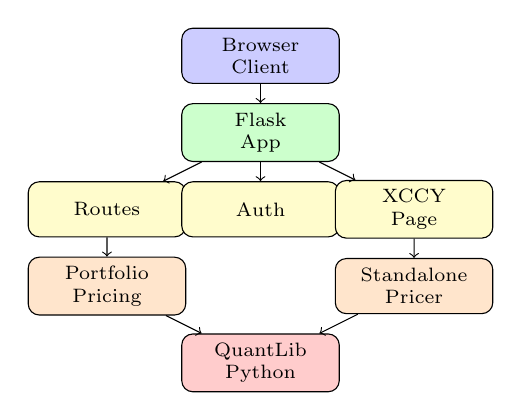
\begin{tikzpicture}[scale=0.65,
    box/.style={rectangle, draw, rounded corners, minimum width=2cm, minimum height=0.7cm, align=center, font=\scriptsize}]

    % Layers
    \node[box, fill=blue!20] (browser) at (0,5) {Browser\\Client};
    \node[box, fill=green!20] (flask) at (0,3.5) {Flask\\App};
    \node[box, fill=yellow!20] (routes) at (-3,2) {Routes};
    \node[box, fill=yellow!20] (auth) at (0,2) {Auth};
    \node[box, fill=yellow!20] (xccy) at (3,2) {XCCY\\Page};
    \node[box, fill=orange!20] (portfolio) at (-3,0.5) {Portfolio\\Pricing};
    \node[box, fill=orange!20] (pricer) at (3,0.5) {Standalone\\Pricer};
    \node[box, fill=red!20] (ql) at (0,-1) {QuantLib\\Python};

    \draw[->] (browser) -- (flask);
    \draw[->] (flask) -- (routes);
    \draw[->] (flask) -- (auth);
    \draw[->] (flask) -- (xccy);
    \draw[->] (routes) -- (portfolio);
    \draw[->] (xccy) -- (pricer);
    \draw[->] (portfolio) -- (ql);
    \draw[->] (pricer) -- (ql);
\end{tikzpicture}
\end{center}
\end{frame}

\begin{frame}{Flask Application Structure}
\textbf{Package: tgir\_quantlib\_tools/}
\begin{itemize}
    \item \texttt{\_\_init\_\_.py} --- Package init, creates app
    \item \texttt{app\_factory.py} --- Flask app factory
    \item \texttt{config.py} --- Environment-based configuration
    \item \texttt{auth.py} --- Session authentication
    \item \texttt{routes.py} --- Main route registration
    \item \texttt{dashboard.py} --- Dashboard views
    \item \texttt{xccy\_page.py} --- XCCY callable interface
\end{itemize}

\textbf{Key Design Patterns:}
\begin{itemize}
    \item Application factory pattern
    \item Blueprint-based route organization
    \item Session-based authentication
    \item JSON state management
\end{itemize}
\end{frame}

\begin{frame}{Proposed REST Contract for System Integration}
\textbf{Specified future API at /api/v1/}

\textbf{Core Endpoints:}
\begin{itemize}
    \item \texttt{POST /api/v1/callable-xccy/validate} --- Validate deal JSON
    \item \texttt{POST /api/v1/callable-xccy/price} --- Synchronous pricing
    \item \texttt{POST /api/v1/callable-xccy/jobs} --- Async job submission
    \item \texttt{GET /api/v1/callable-xccy/jobs/\{id\}} --- Job status/results
    \item \texttt{GET /api/v1/engine} --- Engine info, schemas, limits
\end{itemize}

\textbf{Design Principles:}
\begin{itemize}
    \item No QuantLib/Python types cross REST boundary
    \item JSON input/output with schema validation
    \item mTLS authentication for production
    \item Idempotent operations with retry support
\end{itemize}

\textbf{Status:} Detailed integration specification; these Flask endpoints are not yet implemented.
\end{frame}

\begin{frame}{Model Context Protocol (MCP)}
\textbf{File: xccy\_pricer\_mcp.py}

\textbf{What is MCP?}
\begin{itemize}
    \item Protocol for exposing structured tools
    \item Used by AI assistants (Claude, etc.)
    \item JSON-RPC over stdio or HTTP
\end{itemize}

\textbf{Exposed Tools:}
\begin{itemize}
    \item \texttt{xccy\_validate\_deal} --- Validate market and deal inputs
    \item \texttt{xccy\_price\_deal} --- Validate and price one deal
\end{itemize}

\textbf{Use Case:} AI-assisted pricing queries via Claude, GPT, etc.
\end{frame}

\begin{frame}{Integration Summary: REST + MCP}
\begin{center}
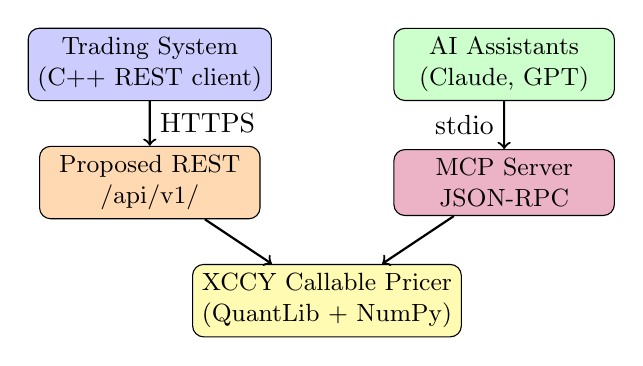
\begin{tikzpicture}[scale=0.75,
    box/.style={rectangle, draw, rounded corners, minimum width=2.8cm, minimum height=0.8cm, align=center, font=\small}]

    \node[box, fill=blue!20] (trading) at (-3,2) {Trading System\\(C++ REST client)};
    \node[box, fill=green!20] (ai) at (3,2) {AI Assistants\\(Claude, GPT)};
    \node[box, fill=orange!30] (rest) at (-3,0) {Proposed REST\\/api/v1/};
    \node[box, fill=purple!30] (mcp) at (3,0) {MCP Server\\JSON-RPC};
    \node[box, fill=yellow!30] (pricer) at (0,-2) {XCCY Callable Pricer\\(QuantLib + NumPy)};

    \draw[->, thick] (trading) -- (rest) node[midway, right] {HTTPS};
    \draw[->, thick] (ai) -- (mcp) node[midway, left] {stdio};
    \draw[->, thick] (rest) -- (pricer);
    \draw[->, thick] (mcp) -- (pricer);
\end{tikzpicture}
\end{center}

\textbf{Both interfaces expose the same pricer:}
\begin{itemize}
    \item \textbf{REST contract:} Specified for future trading-system and batch integration
    \item \textbf{MCP:} Implemented for LLM integration and AI-assisted analysis
\end{itemize}
\end{frame}

\begin{frame}{DigitalOcean Deployment Architecture}
\textbf{Infrastructure:} Single DigitalOcean Droplet

\begin{center}
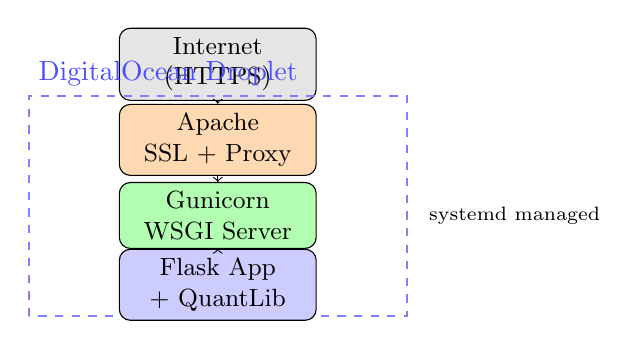
\begin{tikzpicture}[scale=0.8,
    box/.style={rectangle, draw, rounded corners, minimum width=2.5cm, minimum height=0.7cm, align=center, font=\small}]

    % Internet
    \node[box, fill=gray!20] (inet) at (0,4) {Internet\\(HTTPS)};

    % DigitalOcean droplet boundary
    \draw[dashed, thick, blue!50] (-3,0) rectangle (3,3.5);
    \node[anchor=south west, blue!70] at (-3,3.5) {DigitalOcean Droplet};

    % Components
    \node[box, fill=orange!30] (apache) at (0,2.8) {Apache\\SSL + Proxy};
    \node[box, fill=green!30] (gunicorn) at (0,1.6) {Gunicorn\\WSGI Server};
    \node[box, fill=blue!20] (flask) at (0,0.5) {Flask App\\+ QuantLib};

    % Arrows
    \draw[->] (inet) -- (apache);
    \draw[->] (apache) -- (gunicorn);
    \draw[->] (gunicorn) -- (flask);

    % systemd label
    \node[anchor=west, font=\scriptsize] at (3.2,1.6) {systemd managed};
\end{tikzpicture}
\end{center}

\textbf{Specifications:}
\begin{itemize}
    \item Basic Droplet: 2GB RAM, 1 vCPU (\$7/month --- hobby-friendly!)
    \item Ubuntu 22.04 LTS
    \item Let's Encrypt SSL certificates
\end{itemize}
\end{frame}

\begin{frame}{DigitalOcean Deployment Steps}
\textbf{1. Create Droplet:}
\begin{itemize}
    \item Select Ubuntu 22.04 LTS image
    \item Choose Basic plan (\$7/month for 2GB RAM)
    \item Add SSH key for secure access
    \item Select region (e.g., NYC3)
\end{itemize}

\textbf{2. Install Dependencies:}
\begin{itemize}
    \item \texttt{apt install python3.11 python3-venv apache2}
    \item \texttt{pip install gunicorn flask quantlib-python}
    \item Enable mod\_proxy, mod\_ssl for Apache
\end{itemize}

\textbf{3. Configure Services:}
\begin{itemize}
    \item Copy \texttt{deploy/systemd/*.template} $\to$ \texttt{/etc/systemd/system/}
    \item Copy \texttt{deploy/apache/*.template} $\to$ \texttt{/etc/apache2/sites-available/}
    \item Run \texttt{certbot --apache} for SSL
\end{itemize}

\textbf{4. Start Application:}
\begin{itemize}
    \item \texttt{systemctl enable --now tgir-quantlib-tools}
\end{itemize}
\end{frame}

\begin{frame}{Production Configuration Files}
\textbf{systemd Service:} \texttt{/etc/systemd/system/tgir-quantlib-tools.service}
\begin{itemize}
    \item \texttt{WorkingDirectory=/opt/tgir-quantlib-tools}
    \item \texttt{ExecStart=/opt/.venv/bin/gunicorn -w 2 -b 127.0.0.1:8000 wsgi:app}
    \item \texttt{Restart=always}
\end{itemize}

\textbf{Apache VirtualHost:}
\begin{itemize}
    \item SSL termination (port 443)
    \item Redirect HTTP $\to$ HTTPS
    \item \texttt{ProxyPass / http://127.0.0.1:8000/}
\end{itemize}

\textbf{Environment Variables:} \texttt{/opt/tgir-quantlib-tools/.env}
\begin{itemize}
    \item \texttt{FLASK\_SECRET\_KEY=<random>}
    \item \texttt{APP\_USERNAME=admin}
    \item \texttt{APP\_PASSWORD\_HASH=<bcrypt>}
\end{itemize}

\textbf{CI/CD:}
\begin{itemize}
    \item GitHub Actions: test on push, deploy on tag
    \item SSH deployment via GitHub Secrets
\end{itemize}
\end{frame}

\begin{frame}{Security Considerations}
\textbf{Authentication:}
\begin{itemize}
    \item Environment-variable credentials
    \item Session-based login
    \item Debug mode fallback (local only)
\end{itemize}

\textbf{Input Validation:}
\begin{itemize}
    \item Schema validation for all JSON
    \item Type checking on all fields
    \item Range checks for numerics
    \item Positive semi-definiteness for correlation
\end{itemize}

\textbf{Error Handling:}
\begin{itemize}
    \item Custom \texttt{PricingError} exception
    \item Detailed error messages
    \item No internal state exposure
\end{itemize}
\end{frame}

\begin{frame}{Model Limitations}
\textbf{Documented Limitations:}
\begin{enumerate}
    \item Rate volatility is one-piece constant per currency
    \item Forecast/discount basis is deterministic
    \item FX uses ATM lognormal (no smile)
    \item EUR overnight uses continuous approximation
    \item LSM is a lower bound (no dual/upper bound)
\end{enumerate}

\textbf{Appropriate Use:}
\begin{itemize}
    \item Research and education
    \item Indicative pricing
    \item Model validation testing
\end{itemize}

\textbf{NOT for:}
\begin{itemize}
    \item Production trading systems
    \item Regulatory capital calculations
    \item Client-facing quotes
\end{itemize}
\end{frame}

%%%%%%%%%%%%%%%%%%%%%%%%%%%%%%%%%%%%%%%%%%%%%%%%%%%%%%%%%%%%%%%%%%%%%%%%%%%%%%%%
%% PART 8: SUMMARY AND FUTURE WORK (Slides 196-200)
%%%%%%%%%%%%%%%%%%%%%%%%%%%%%%%%%%%%%%%%%%%%%%%%%%%%%%%%%%%%%%%%%%%%%%%%%%%%%%%%

\begin{frame}{}
\begin{center}
\Huge\textbf{Part VIII}\\[1cm]
\Large Summary and Future Work
\end{center}
\end{frame}

\begin{frame}{What We Built}
\textbf{Core Deliverables:}
\begin{enumerate}
    \item SOFR curve bootstrap with full OIS strip
    \item Hull-White and G2++ swaption calibration
    \item European and Bermudan swaption pricing
    \item Equity cliquet pricing with Greeks
    \item \textbf{Three-factor callable XCCY pricer}
    \item Comprehensive validation test suite
    \item Flask web application
    \item MCP server for AI integration
\end{enumerate}

\textbf{Lines of Code:}
\begin{itemize}
    \item standalone\_xccy\_pricer.py: 1,400+ lines
    \item portfolio.py: 1,000+ lines
    \item Test files: 500+ lines
    \item Total: 3,000+ lines of Python
\end{itemize}
\end{frame}

\begin{frame}{Key Technical Achievements}
\begin{enumerate}
    \item \textbf{Correct Three-Factor Dynamics:}
    \begin{itemize}
        \item Proper quanto drift adjustment
        \item Exact Gaussian state evolution
        \item Validated martingale conditions
    \end{itemize}

    \item \textbf{Robust Calibration:}
    \begin{itemize}
        \item OIS curves to 0.01bp accuracy
        \item Swaption fit $<$5\% RMS
        \item FX vol fit $<$25bp
    \end{itemize}

    \item \textbf{Efficient Monte Carlo:}
    \begin{itemize}
        \item 30,000 paths in $\sim$10 seconds
        \item Antithetic variance reduction
        \item Two-pass LSM for unbiased pricing
    \end{itemize}

    \item \textbf{Comprehensive Testing:}
    \begin{itemize}
        \item 20 validation tests
        \item Structural bounds, monotonicity, convergence
    \end{itemize}
\end{enumerate}
\end{frame}

\begin{frame}{Future Enhancements}
\textbf{Model Extensions:}
\begin{itemize}
    \item Piecewise constant rate volatility
    \item Stochastic basis spreads
    \item FX smile/skew calibration
    \item Multi-curve framework
\end{itemize}

\textbf{Numerical Improvements:}
\begin{itemize}
    \item Dual/upper bound implementation
    \item Quasi-Monte Carlo (Sobol sequences)
    \item GPU acceleration (CuPy)
    \item Automatic differentiation for Greeks
\end{itemize}

\textbf{Production Features:}
\begin{itemize}
    \item Real-time market data feeds
    \item Risk aggregation
    \item Audit trails and controls
    \item Regulatory reporting
\end{itemize}
\end{frame}

\begin{frame}{Key Takeaways}
\begin{enumerate}
    \item \textbf{QuantLib is powerful} but has limits for exotic structures

    \item \textbf{Python + NumPy} is viable for research/prototype pricing

    \item \textbf{Validation is critical:} martingales, bounds, convergence

    \item \textbf{Three-factor models} add significant complexity:
    \begin{itemize}
        \item Quanto adjustments
        \item Correlation constraints
        \item State dimension management
    \end{itemize}

    \item \textbf{LSM provides lower bound} --- always document limitations

    \item \textbf{Good testing} catches bugs early

    \item \textbf{Documentation} enables knowledge transfer
\end{enumerate}
\end{frame}

%%%%%%%%%%%%%%%%%%%%%%%%%%%%%%%%%%%%%%%%%%%%%%%%%%%%%%%%%%%%%%%%%%%%%%%%%%%%%%%%
%% COLLABORATIVE AI DEVELOPMENT METHODOLOGY
%%%%%%%%%%%%%%%%%%%%%%%%%%%%%%%%%%%%%%%%%%%%%%%%%%%%%%%%%%%%%%%%%%%%%%%%%%%%%%%%

\begin{frame}{}
\begin{center}
\Huge\textbf{Appendix}\\[1cm]
\Large Collaborative AI Development\\[0.5cm]
\normalsize A Methodology as Important as the Model Itself
\end{center}
\end{frame}

\begin{frame}{The Collaborative Development Ecosystem}
\textbf{This project was built by human + AI collaboration:}

\begin{center}
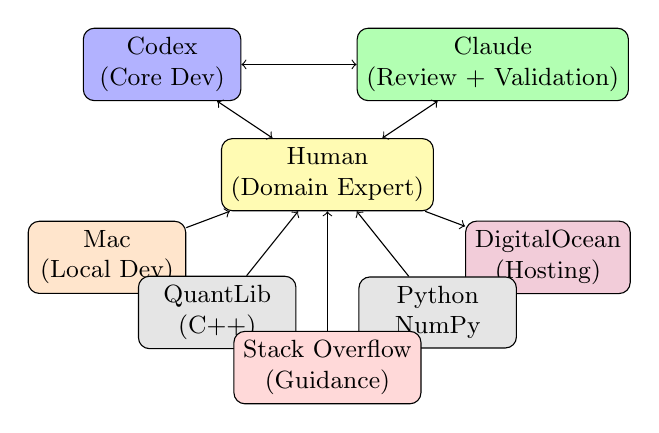
\begin{tikzpicture}[scale=0.7,
    box/.style={rectangle, draw, rounded corners, minimum width=2cm, minimum height=0.6cm, align=center, font=\small}]

    % Human at center
    \node[box, fill=yellow!30, minimum width=2.5cm] (human) at (0,0) {Human\\(Domain Expert)};

    % AI Agents
    \node[box, fill=blue!30] (codex) at (-3,2) {Codex\\(Core Dev)};
    \node[box, fill=green!30] (claude) at (3,2) {Claude\\(Review + Validation)};

    % Infrastructure
    \node[box, fill=orange!20] (mac) at (-4,-1.5) {Mac\\(Local Dev)};
    \node[box, fill=purple!20] (do) at (4,-1.5) {DigitalOcean\\(Hosting)};

    % Libraries
    \node[box, fill=gray!20] (ql) at (-2,-2.5) {QuantLib\\(C++)};
    \node[box, fill=gray!20] (py) at (2,-2.5) {Python\\NumPy};

    % Resources
    \node[box, fill=red!15] (so) at (0,-3.5) {Stack Overflow\\(Guidance)};

    % Connections
    \draw[<->] (human) -- (codex);
    \draw[<->] (human) -- (claude);
    \draw[<->] (codex) -- (claude);
    \draw[->] (mac) -- (human);
    \draw[->] (human) -- (do);
    \draw[->] (ql) -- (human);
    \draw[->] (py) -- (human);
    \draw[->] (so) -- (human);
\end{tikzpicture}
\end{center}

\textbf{Key Insight:} The collaborative methodology is as significant as the pricer itself
\end{frame}

\begin{frame}{Division of Labor: Codex vs Claude}
\begin{table}
\centering
\begin{tabular}{lll}
\toprule
\textbf{Agent} & \textbf{Primary Role} & \textbf{Deliverables} \\
\midrule
\textbf{Codex} & Core Development & Specifications \\
(OpenAI) & Ground-up programming & Core implementation \\
 & Rigorous specs & Initial test suite \\
\midrule
\textbf{Claude} & Review \& Extension & Code review \\
(Anthropic) & Validation framework & Regression tests \\
 & Quality assurance & Documentation \\
\bottomrule
\end{tabular}
\end{table}

\textbf{Human Role:}
\begin{itemize}
    \item \textbf{Domain expertise:} Financial mathematics, market conventions
    \item \textbf{Orchestration:} Directing agents, integrating outputs
    \item \textbf{Final validation:} Ensuring correctness against theory
\end{itemize}
\end{frame}

\begin{frame}{Codex: Rigorous Specification \& Programming}
\textbf{What Codex Built:}

\begin{enumerate}
    \item \textbf{Formal Specifications:}
    \begin{itemize}
        \item Mathematical model documentation
        \item API contracts and type hints
        \item JSON schemas for inputs/outputs
    \end{itemize}

    \item \textbf{Core Implementation:}
    \begin{itemize}
        \item Three-factor Monte Carlo engine
        \item Longstaff-Schwartz regression
        \item Curve bootstrapping routines
    \end{itemize}

    \item \textbf{Initial Test Suite:}
    \begin{itemize}
        \item Unit tests for each component
        \item Integration tests for full pricing
        \item Property-based test scaffolds
    \end{itemize}
\end{enumerate}

\textbf{Human guidance:} Provided mathematical formulas, QuantLib patterns, market conventions
\end{frame}

\begin{frame}{Claude: Code Review \& Validation Framework}
\textbf{What Claude Built:}

\begin{enumerate}
    \item \textbf{Code Review:}
    \begin{itemize}
        \item Reviewed Codex's implementations
        \item Identified numerical stability issues
        \item Suggested optimizations
    \end{itemize}

    \item \textbf{Validation Framework (Key Contribution):}
    \begin{itemize}
        \item Martingale test infrastructure
        \item Structural bounds verification
        \item Monotonicity checking
        \item Convergence analysis
    \end{itemize}

    \item \textbf{Regression Testing:}
    \begin{itemize}
        \item Built tests to catch future changes
        \item Automated validation on every commit
        \item Extended Codex's work systematically
    \end{itemize}
\end{enumerate}

\textbf{Critical:} Claude's validation framework provides confidence in correctness
\end{frame}

\begin{frame}{The Collaborative Workflow}
\begin{center}
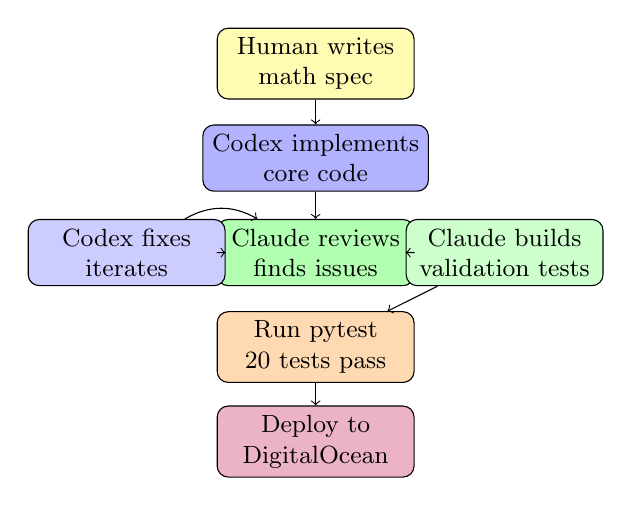
\begin{tikzpicture}[scale=0.8,
    box/.style={rectangle, draw, rounded corners, minimum width=2.5cm, minimum height=0.7cm, align=center, font=\small}]

    \node[box, fill=yellow!30] (spec) at (0,4) {Human writes\\math spec};
    \node[box, fill=blue!30] (codex) at (0,2.5) {Codex implements\\core code};
    \node[box, fill=green!30] (review) at (0,1) {Claude reviews\\finds issues};
    \node[box, fill=blue!20] (fix) at (-3,1) {Codex fixes\\iterates};
    \node[box, fill=green!20] (valid) at (3,1) {Claude builds\\validation tests};
    \node[box, fill=orange!30] (run) at (0,-0.5) {Run pytest\\20 tests pass};
    \node[box, fill=purple!30] (deploy) at (0,-2) {Deploy to\\DigitalOcean};

    \draw[->] (spec) -- (codex);
    \draw[->] (codex) -- (review);
    \draw[->] (review) -- (fix);
    \draw[->] (review) -- (valid);
    \draw[->] (fix) to[bend left] (review);
    \draw[->] (valid) -- (run);
    \draw[->] (run) -- (deploy);
\end{tikzpicture}
\end{center}

\textbf{Iteration:} Multiple cycles between Codex implementation and Claude validation
\end{frame}

\begin{frame}{Zero-Intervention Automation Pipeline}
\textbf{A Hobby Project with Rigorous Engineering:}

One prompt triggers the \textbf{entire pipeline} with no human intervention:

\begin{enumerate}
    \item \textcolor{blue!70}{\textbf{Coding}} --- AI implements from specs
    \item \textcolor{orange!70}{\textbf{Regression Testing}} --- pytest runs 20+ tests locally
    \item \textcolor{purple!70}{\textbf{Browser UI Testing}} --- Playwright validates Flask UI
    \item \textcolor{green!70}{\textbf{Documentation}} --- LaTeX and markdown auto-updated
    \item \textcolor{gray!70}{\textbf{Local Run}} --- Optional manual verification
    \item \textcolor{cyan!70}{\textbf{Deploy to DigitalOcean}} --- SSH + Git pull + systemd restart
    \item \textcolor{orange!70}{\textbf{Production Regression}} --- Tests run on production
    \item \textcolor{red!70}{\textbf{Telegram Notification}} --- ``Deployment complete!''
\end{enumerate}

\vspace{0.3cm}
\begin{center}
\fbox{\parbox{0.9\textwidth}{
\textbf{Key Insight:} This is a \textit{hobby project} costing \$7/month --- but it's built with the same rigor as production systems at top tech companies.
}}
\end{center}
\end{frame}

\begin{frame}{Extended Technology Stack}
\textbf{The Full Ecosystem:}

\begin{table}
\centering
\small
\begin{tabular}{lll}
\toprule
\textbf{Component} & \textbf{Role} & \textbf{Integration} \\
\midrule
Mac (local) & Development environment & VS Code, terminal \\
DigitalOcean & Production hosting & Apache, Gunicorn \\
\midrule
Codex (OpenAI) & Core development & Specs, implementation \\
Claude (Anthropic) & Review \& validation & Tests, extensions \\
GitHub Copilot & Inline assistance & VS Code integration \\
\midrule
QuantLib (C++) & Foundation library & Curves, calibration \\
Python 3.13 & Primary language & NumPy, Flask \\
Stack Overflow & Guidance verification & Edge cases, patterns \\
\bottomrule
\end{tabular}
\end{table}

\textbf{Cohesion:} All components work together in a unified workflow
\end{frame}

\begin{frame}{QuantLib Extension with AI Assistance}
\textbf{Where QuantLib Fell Short:}
\begin{itemize}
    \item No native callable XCCY support
    \item Limited multi-currency Monte Carlo
    \item No built-in LSM for XCCY
\end{itemize}

\textbf{How We Extended It (AI-Assisted):}
\begin{enumerate}
    \item \textbf{Codex:} Wrote custom Monte Carlo engine using QuantLib curves
    \item \textbf{Claude:} Verified QuantLib API usage against documentation
    \item \textbf{Stack Overflow:} Confirmed edge cases and patterns
    \item \textbf{Human:} Ensured extensions followed QuantLib conventions
\end{enumerate}

\textbf{Result:} 1,400+ lines of rigorous custom code that extends QuantLib capabilities

\textbf{Principle:} Use QuantLib for what it does well, extend rigorously where needed
\end{frame}

\begin{frame}{Why This Methodology Matters}
\begin{enumerate}
    \item \textbf{Quality Through Collaboration:}
    \begin{itemize}
        \item Two AI agents catch each other's errors
        \item Human provides domain grounding
        \item Stack Overflow validates edge cases
    \end{itemize}

    \item \textbf{Rigorous by Design:}
    \begin{itemize}
        \item Codex writes specs before code
        \item Claude builds validation before deployment
        \item 20 automated tests provide safety net
    \end{itemize}

    \item \textbf{Reproducible Workflow:}
    \begin{itemize}
        \item Same methodology can build other pricers
        \item Pattern: Codex $\to$ Claude $\to$ Human validation
        \item Infrastructure (Mac + DigitalOcean) reusable
    \end{itemize}
\end{enumerate}

\fbox{\parbox{0.9\textwidth}{\centering The collaborative methodology is as valuable as the callable XCCY pricer itself}}
\end{frame}

\begin{frame}{Lessons Learned: Human + AI Collaboration}
\begin{enumerate}
    \item \textbf{Specialization works:}
    \begin{itemize}
        \item Codex for ground-up development
        \item Claude for review and validation
        \item Human for domain expertise and orchestration
    \end{itemize}

    \item \textbf{Validation is critical:}
    \begin{itemize}
        \item Claude's test framework caught bugs Codex missed
        \item Regression tests prevent future breakage
        \item Never trust single-agent output
    \end{itemize}

    \item \textbf{Stack Overflow still matters:}
    \begin{itemize}
        \item AI can hallucinate APIs
        \item Human experts catch edge cases
        \item Community knowledge validates approaches
    \end{itemize}

    \item \textbf{Infrastructure enables iteration:}
    \begin{itemize}
        \item Mac for rapid local development
        \item DigitalOcean for deployment testing
        \item pytest for automated validation
    \end{itemize}
\end{enumerate}
\end{frame}

\begin{frame}{Questions and Discussion}
\begin{center}
\Huge Thank You!\\[1cm]
\Large Questions?\\[1cm]
\normalsize
Repository: \texttt{tgir\_quantlib\_tools}\\
Model ID: \texttt{HW1F\_USD\_HW1F\_EUR\_BSFX\_LSM\_V1}
\end{center}
\end{frame}

\end{document}
